

\documentclass[11pt,aspectratio=1610]{beamer}	% Available font sizes 8pt, 9pt, 10pt, 11pt, 12pt, 14pt, 17pt, 20pt. Default font size 11pt (corresponds to 22pt at the full screen mode)
\usepackage[utf8]{inputenc}
% 16:10 -> 160x100mm
% 4:3 native slide format 128mm x 96mm

\usetheme{Darmstadt}
\usecolortheme{beaver}
\setbeamercolor{title}{fg=blue}

% \setbeamertemplate{footline}[page number]
% \setbeamertemplate{footline}[frame number]
% \setbeamertemplate{footline}{\hfill\strut\insertframenumber\quad\quad}
% \setbeamertemplate{footline}{\hfill\strut\footnotesize\insertpagenumber\quad\quad}
\setbeamertemplate{navigation symbols}{\insertslidenavigationsymbol\insertbackfindforwardnavigationsymbol\quad\hfill\strut\footnotesize\insertframenumber\quad}

\usepackage{natbib}	%defines citation style
% \citestyle{aa}

\usepackage{caption}
\captionsetup[figure]{labelformat=empty,singlelinecheck=false,aboveskip=1pt,justification=raggedright,font=scriptsize}
\newcommand{\captionoftiny}[2]{\captionof{#1}{\color{gray} \tiny #2}}

\setbeamercolor{button}{bg=white,fg=gray}

\usepackage{siunitx}
	\DeclareSIUnit[number-unit-product=\,]\au{au}
	\DeclareSIUnit[number-unit-product=\,]\nT{\nano\tesla}
	\DeclareSIUnit[number-unit-product=\,]\Rs{\textit{R}_\sun{}}
	\DeclareSIUnit[number-unit-product=\,]\RE{\textit{R}_E}
	\sisetup{table-figures-uncertainty=2, table-number-alignment=center, range-phrase=--, range-units=single}

\mode<handout>{
	\usepackage{pgfpages}
	\pgfpagesuselayout{16 on 1}[a4paper,border shrink=8mm,landscape]

	\setbeamercolor{background canvas}{bg=black!2}
}


% maltes_commands.tex
% full journal name replacement
\def\aj{{Astron.~J.}}				%\def\aj{{AJ}}
\def\araa{{Ann.~Rev.~Astron.~Astrophys.}}	%\def\araa{{ARA\&A}}
\def\apj{{Astrophys.~J.}}			%\def\apj{{ApJ}}
\def\apjl{{Astrophys.~J.,~Lett.}}		%\def\apjl{{ApJ}}
\def\mnras{{Mon.~Not.~R.~Astron.~Soc.}}		%\def\mnras{{MNRAS}}
\def\aap{{Astron.~Astrophys.}}			%\def\aap{{A\&A}}
\def\nat{{Nature}}				%\def\nat{{Nat}}
\def\apjs{{Astrophys.~J.,~Suppl.~Ser.}}		%\def\apjs{{ApJS}}
\def\pasp{{Publ.~Astron.~Soc.~Pac.}}		%\def\pasp{{PASP}}

% other short commands
\def\ion#1#2{{\rm #1}{\sc #2}}
\newcommand{\Hi}{\ion{H}{i}}
\newcommand{\Hii}{\ion{H}{ii}}

% new since 2015
\def\planss{{Planet.~Space~Sci.}}		%Planetary and Space Science
\def\grl{{Geophys.~Res.~Lett.}}			%Geophysical Research Letters
\def\ssr{{Space~Sci.~Rev.}}			%Space Science Reviews
\def\jgr{{J.~Geophys.~Res.}}			%Journal of Geophysical Research

% new since 2016-10-20
\newcommand{\Rsun}{$R_\odot$}
\def\solphys{{Solar~Phys.}}			%\def\solphys{{SoPh}}	%Solar Physics
\def\aapr{{Astron.~Astrophys.~Rev.}}		%\def\aapr{{A\&ARv}}	%The Astronomy and Astrophysics Review

% new since 2017-10-05
\newcommand{\Kp}{\textit{Kp}}

% new since 2017-11-04
\def\zap{{Z.~Astrophys.}}			%\def\zap{{ZAp}}	%Zeitschrift für Astrophysik
\def\procspie{{Proc.~SPIE}}			%Proceedings of the SPIE

% new since 2017-11-16
\def\qjras{{Quart.~J.~R.~Astron.~Soc.}}		%\def\qjras{{QJRAS}}	%Quarterly Journal of the Royal Astronomical Society

% new since 2018-01-28
\newcommand*{\sun}{\ensuremath{\odot}}
\newcommand{\Rs}{$R_\sun{}$}

\newcommand{\vBz}{$vB_\text{z}$}

% new since 2018-04-07
\newcommand{\RE}{$R_\text{E}$}		%\Re already exists...

% new since 2018-06-16
\def\rsquo{{'}}
\def\aaps{{Astron.~Astrophys.,~Suppl.~Ser.}}	%\def\aap{{A\&AS}}	%Astronomy and Astrophysics Supplement Series

% new since 2018-07-29
% get abbreviations from NLM catalog: https://www.ncbi.nlm.nih.gov/nlmcatalog
% search and replace the following abbreviations
% \def\jgra{{J.~Geophys.~Res.~Space~Phys.}}	%Journal of Geophysical Research (Space Physics)
% \def\lrsp{{Living~Rev.~Sol.~Phys.}}		%Living Reviews in Solar Physics
% \def\jswsc{{J.~Space~Weather~Space~Clim.}}	%Journal of Space Weather and Space Climate



% title slide
\title[Solar wind]{The solar wind's geomagnetic impact and its Sun–Earth evolution}
\subtitle{Predictive models for space weather and for the Parker Solar Probe orbit}
% \title[Solar wind]{Empirical solar wind model for the inner heliosphere}
% \subtitle{Predictions for the Parker Solar Probe orbit}
\author[MV]{PhD defense by\\\textit{Malte Venzmer}}
\institute[IAG]{
	\begin{columns}[c]
	\column{0.1\textwidth}
	\column{0.4\textwidth}

		PhD student\\
		within the doctoral program ProPhys,\\
		Georg-August University School of Science (GAUSS)\\
		\ \\
		Institute for Astrophysics\\
		Georg-August-Universität Göttingen

	\column{0.1\textwidth}
	\column{0.4\textwidth}

		\underline{Examination board members}\\
		Dr. Volker Bothmer (supervisor, referee)\\
		Prof. Dr. Ansgar Reiners (2nd referee)\\
		Prof. Dr. Stefan Dreizler\\
		Prof. Dr. Wolfram Kollatschny\\
		Prof. Dr. Hardi Peter\\
		Prof. Dr. Andreas Tilgner
	\end{columns}
	\vspace*{0.2cm}
}
% \date{\today}
\date[2018]{Thursday, 1 November 2018, 14:00\\Seminarraum Astrophysik (SR 17, F 05.104)}
\subject{Solar wind}
% \logo{
\includegraphics[height=1cm]{../talk_figures/IAG_LogoRGB.png}}


\begin{document}

\AtBeginSection[]{
	\subsection{}	% for making the nav dots appear
% 	\frame{\tableofcontents[currentsection]}
}


\section{Title}

\frame[plain]{\titlepage}

\begin{frame}[plain,c]{The two studies in my thesis}{}
	Thesis title:
	\begin{block}{}
		\color{blue} \centering \Large The solar wind's geomagnetic impact and its Sun–Earth evolution\\
		\large Predictive models for space weather and for the Parker Solar Probe orbit
	\end{block}
	
	\begin{columns}[t]
	\column{0.5\textwidth}
		
		\begin{block}<2->{Geomagnetic impact of the solar wind}
			I derived relations to predict geomagnetic activity from
			\begin{itemize}
				\item Solar wind electric field
				\item Velocity of coronal mass ejections
				\item Velocity of solar wind streams
			\end{itemize}
		\end{block}
		
	\column{0.5\textwidth}
		
		\begin{block}<2->{Empirical solar wind model}
			I use existing solar wind data to derive
			\begin{itemize}
				\item Solar wind model for the inner heliosphere
				\item Extrapolation to the near-Sun region
				\item Prediction for Parker Solar Probe orbit
			\end{itemize}
		\end{block}
	
	\end{columns}
\end{frame}

\begin{frame}[c]{Contents}{}
	\begin{columns}[c]
	\column{0.1\textwidth}

	\column{0.9\textwidth}
		
		\large Introduction
		\begin{itemize}
			\item Solar activity
			\item Solar wind
			\item Parker Solar Probe (PSP)
		\end{itemize}
		\large Empirical solar wind model
		\begin{itemize}
			\item Solar wind model
			\item Prediction to PSP orbit
			\item Comparison with other studies
			\item Summary
			\item Outlook
		\end{itemize}
		
	\end{columns}
\end{frame}

% \begin{frame}[plain,c]{Geomagnetic impact of the solar wind}{}
% 	Solar wind -- solar system bodies\\
% 	CMEs -- geomagnetic storms -- effects\\
% 	Importance of prediction of onset/magnitude\\
% 	The study addresses; deriving predictive models
% \end{frame}
% \begin{frame}[plain,c]{Geomagnetic impact of the solar wind}{}
% 	- \Kp~index\\
% 	- Coupling mechanisms\\
% 	- Reconnection at magnetopause
% \end{frame}
% \begin{frame}[plain,c]{Geomagnetic impact of the solar wind}{}
% 	Relations between the \Kp~index and solar wind parameters:\\\ \\
% 	Electric field proxy (\vBz{})	\hfill	Velocity of CMEs and streams\\\ 
% 	
% 	\begin{columns}[c]
% 	\column{0.5\textwidth}
% 		
% 		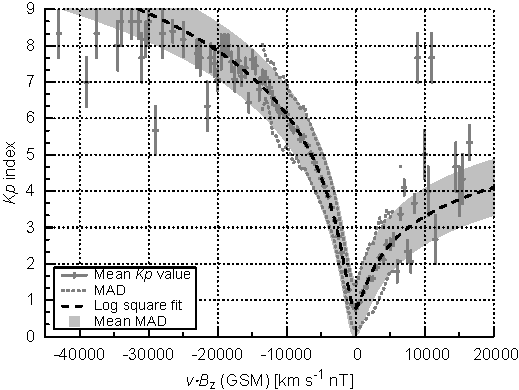
\includegraphics[width=\textwidth]{../figures_of_mine/chapter2/Kp_2dhistogram_VBzgsm_sws_fit_e.pdf}
% 		
% 	\column{0.5\textwidth}
% 	
% 		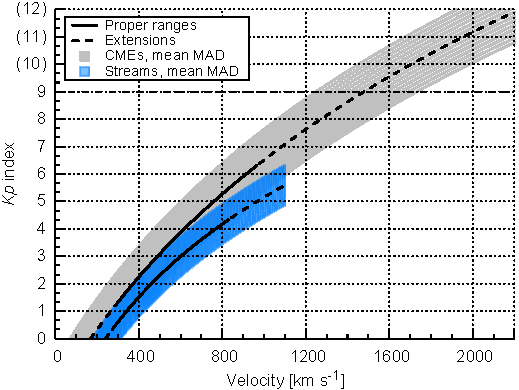
\includegraphics[width=\textwidth]{../figures_of_mine/chapter2/Kp_2dhistogram_V_sws123_fit_f3.pdf}
% 		
% 	\end{columns}
% \end{frame}


\section{Introduction}

\begin{frame}[plain,c]{Solar activity}{}
	\begin{columns}[c]
	\column{0.3\textwidth}
		
		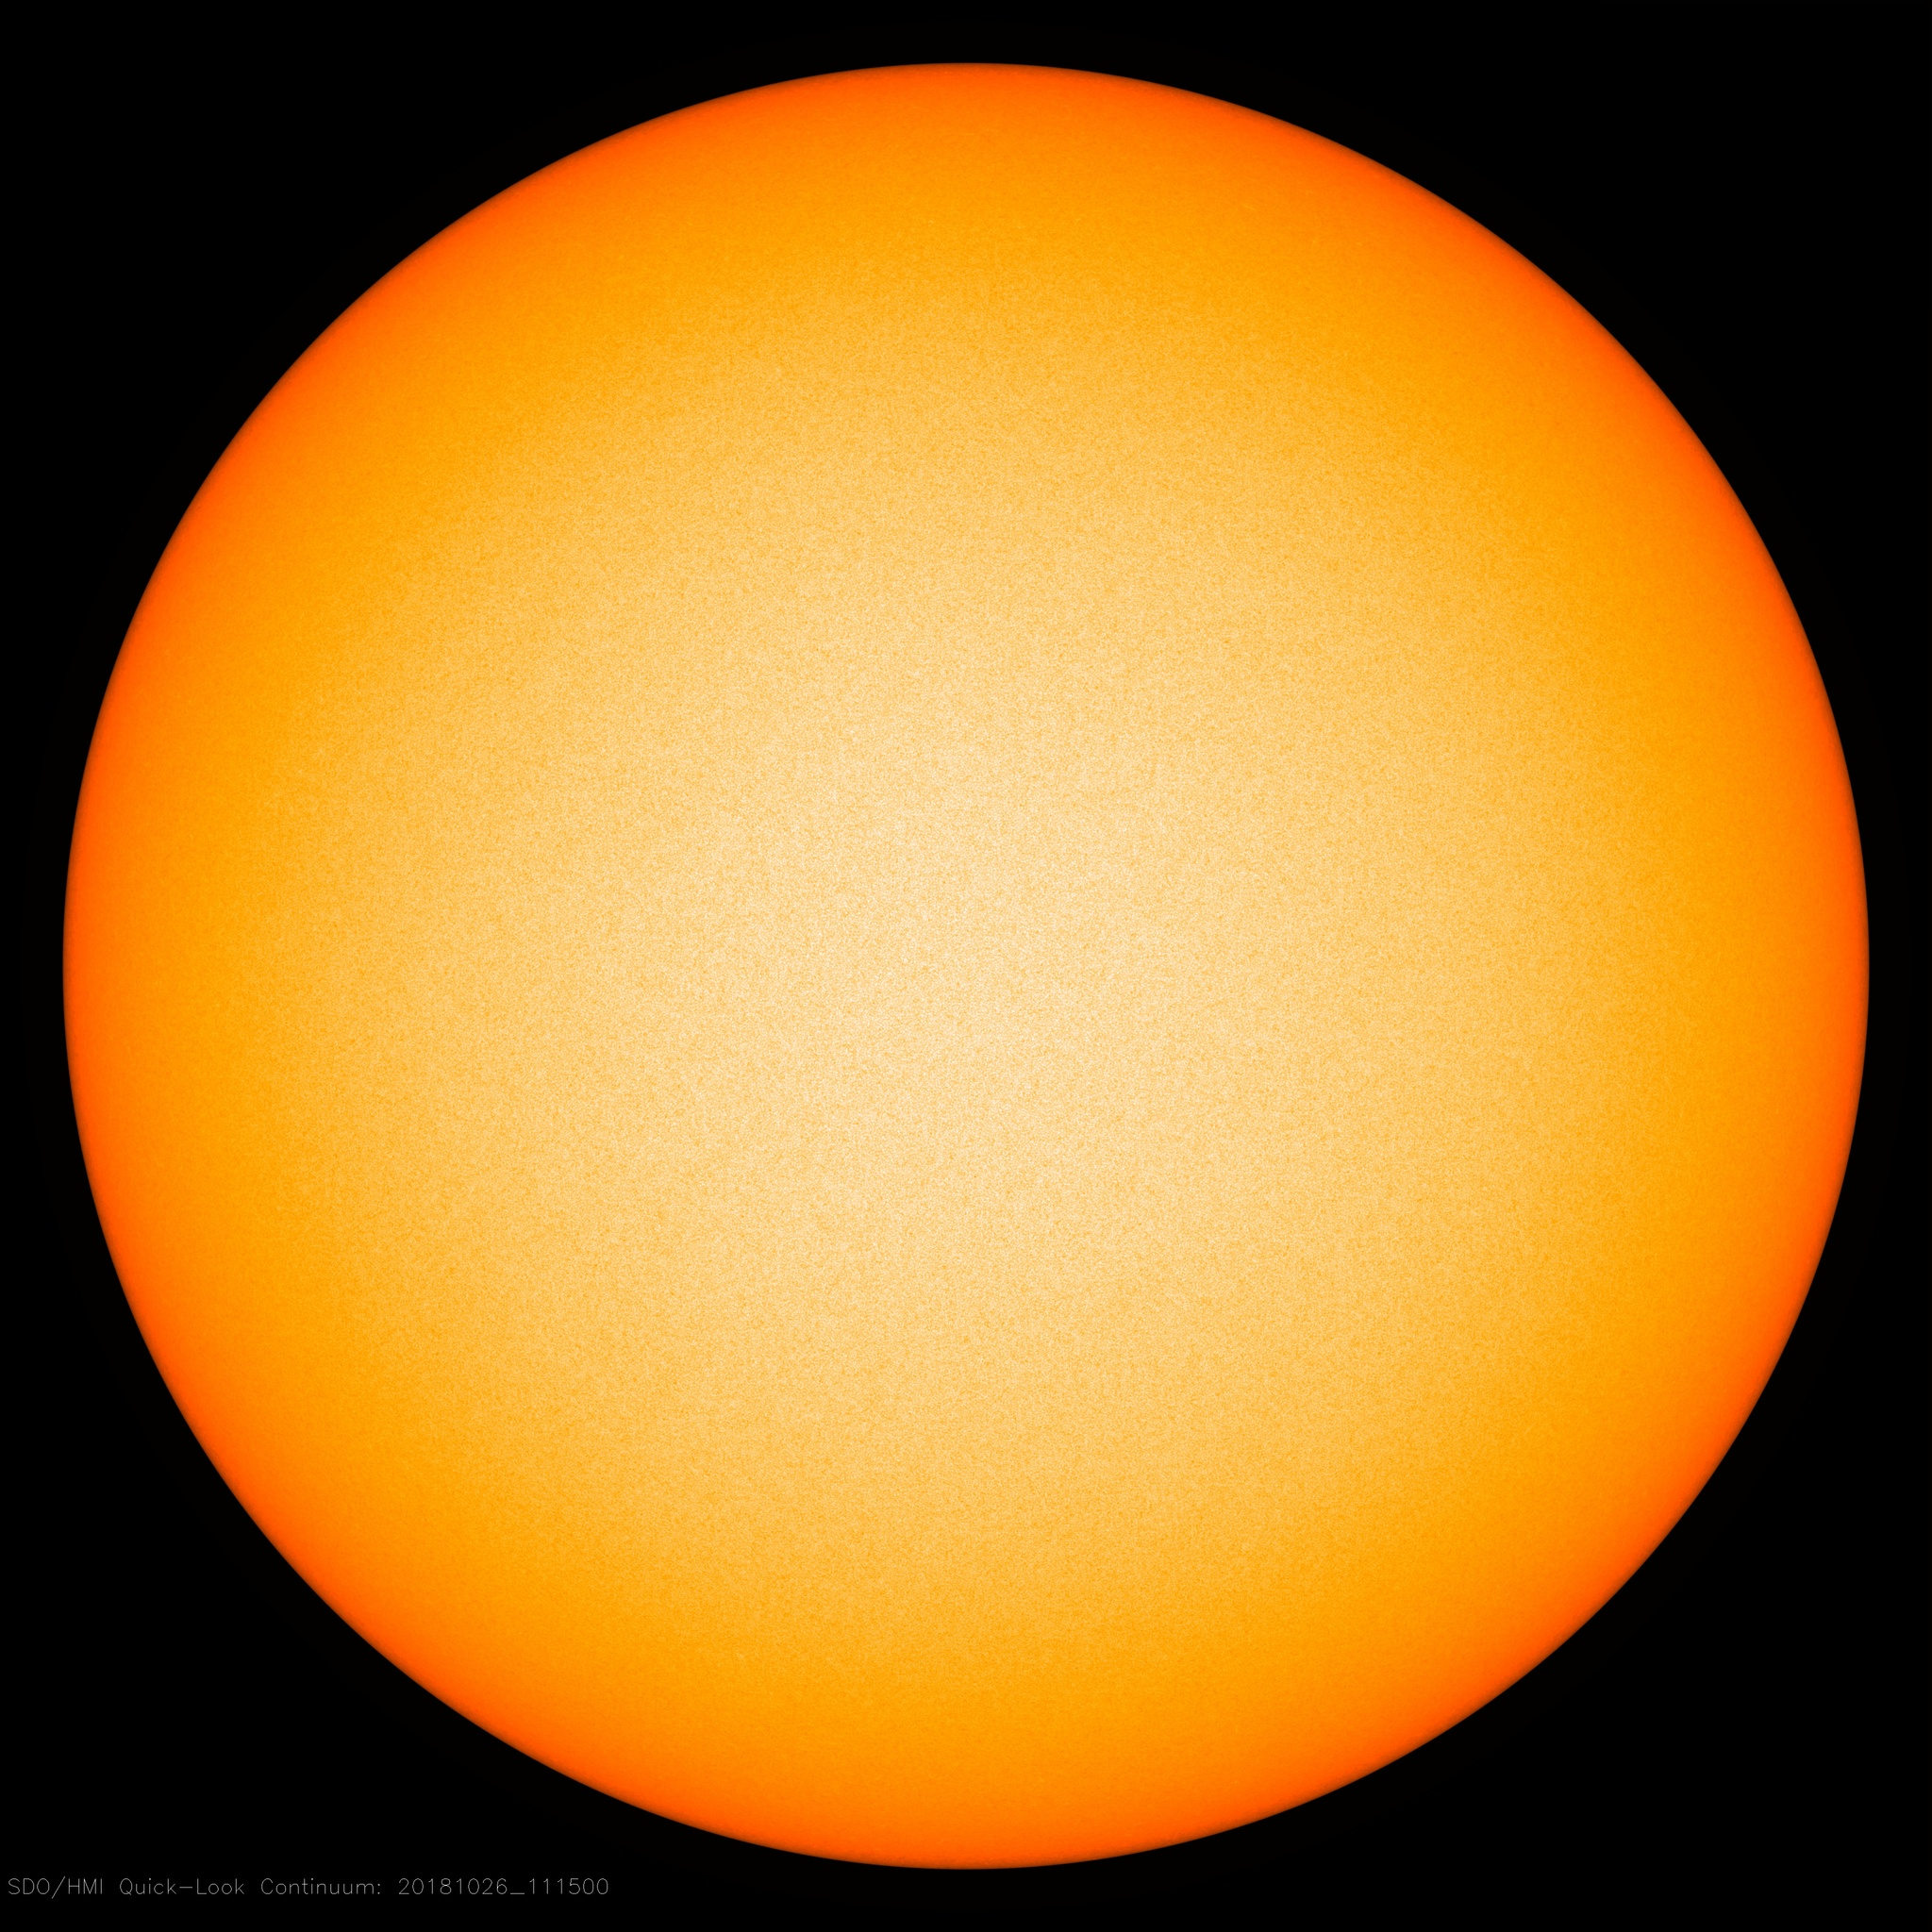
\includegraphics[width=0.96\textwidth]{../talk_figures/latest_2048_HMIIC.jpg}
		\captionoftiny{figure}{\centering Credit: \href{https://sdo.gsfc.nasa.gov/data/}{NASA SDO/HMI}, 26 October 2018}
		\pause
		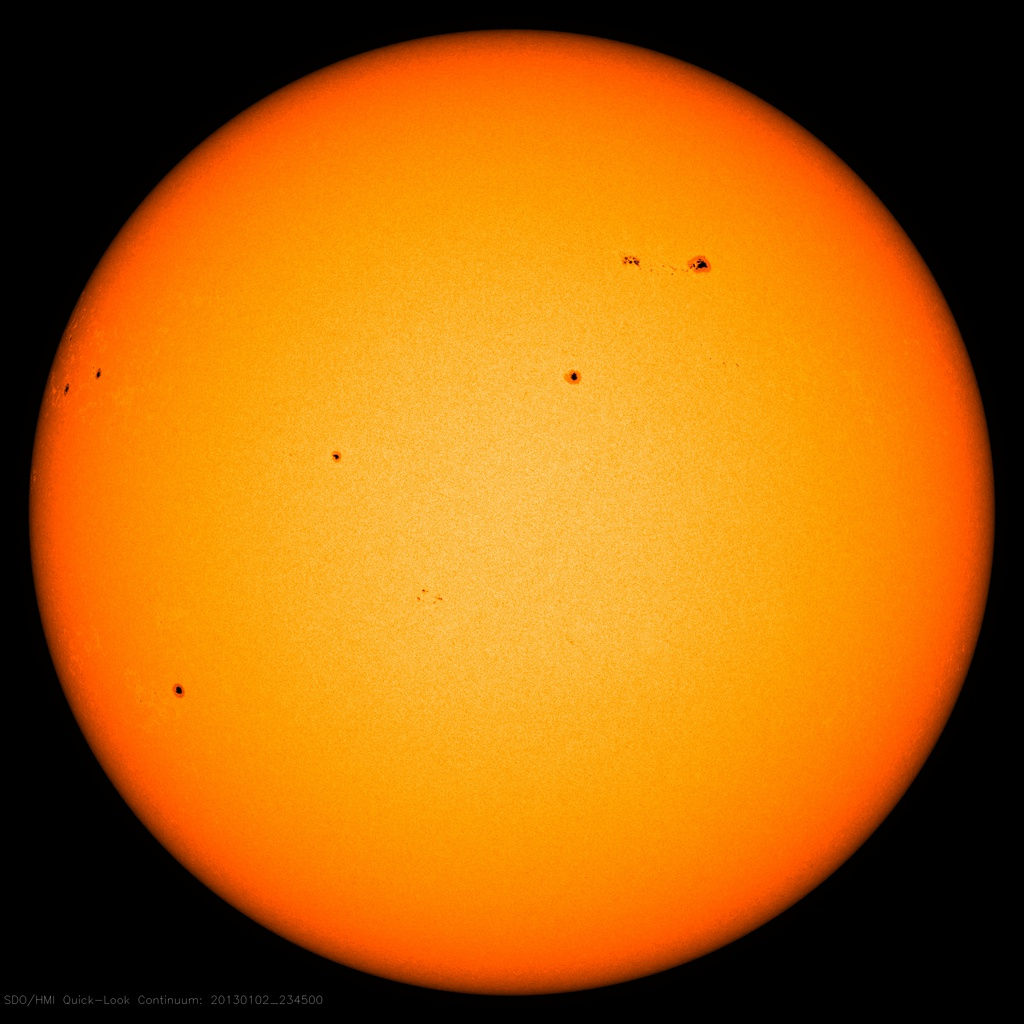
\includegraphics[width=0.96\textwidth]{../talk_figures/20130102_234500_1024_HMIIC.jpg}
		\captionoftiny{figure}{\centering Credit: \href{https://sdo.gsfc.nasa.gov/data/}{NASA SDO/HMI}, 1 January 2013}
		
	\column<3>{0.7\textwidth}
		
		In 1843 the 11-year periodicity was discovered\\\ 
		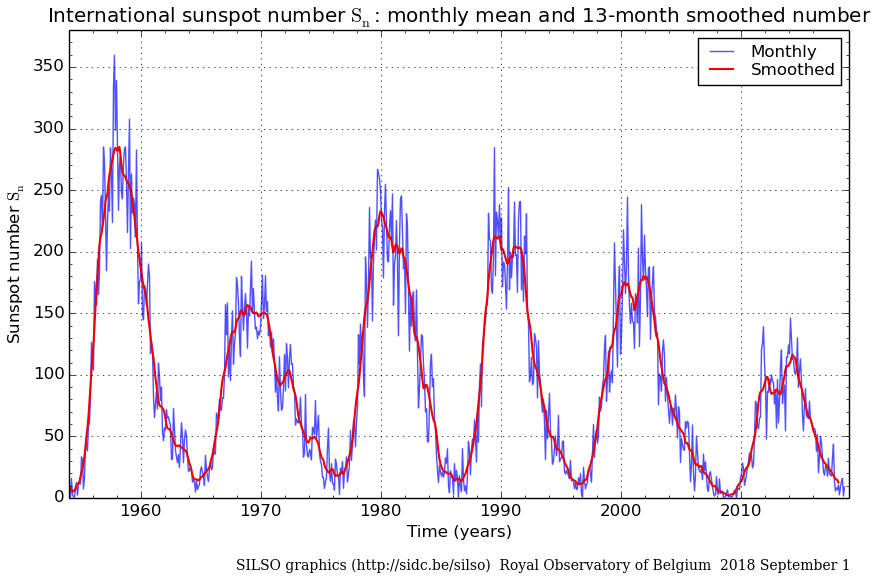
\includegraphics[width=\textwidth]{../figures_of_others/images/ROB_SILSO_SSN_wolfmms_cropped.png}
% 		\captionoftiny{figure}{\centering Credit: \href{http://sidc.be/silso/monthlyssnplot}{SILSO data/image, Royal Observatory of Belgium, Brussels}, 2018}

		\vfill\hfill \hyperlink{butterfly}{\beamerskipbutton{}}
		
	\end{columns}
\end{frame}

\begin{frame}[plain,c]{Solar wind}{}
	\begin{columns}[c]
	\column{\textwidth}
		
		- E.~Parker's theoretical model \citep{Parker1958}\\
		- Confirmation by in-situ measurements in 1959\\
		- Solar wind -- solar system bodies\\
		- Monitored continuously near Earth since\\\ \\
% 		\hspace*{-20pt}
		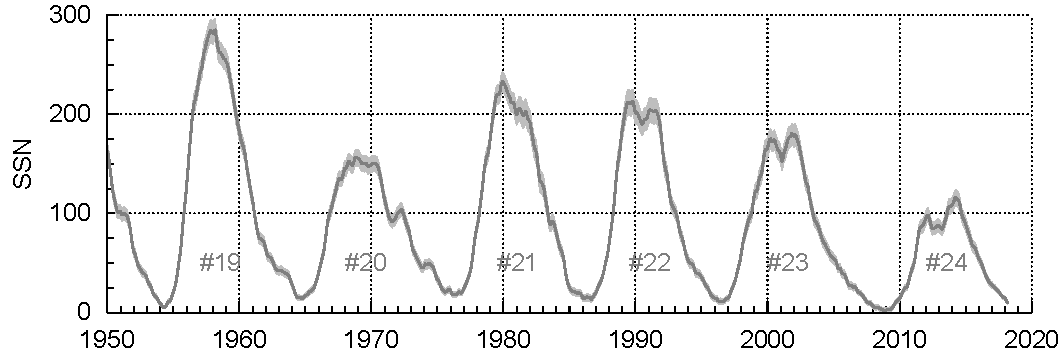
\includegraphics[width=0.7\textwidth]{../talk_figures/timeline_SSN_with_data_and_sc_wosc.pdf}
		\captionoftiny{figure}{\centering Credit: Malte Venzmer, 2018}
		
	\end{columns}
\end{frame}
\begin{frame}[plain,c]{Solar wind}{}
	\centering
	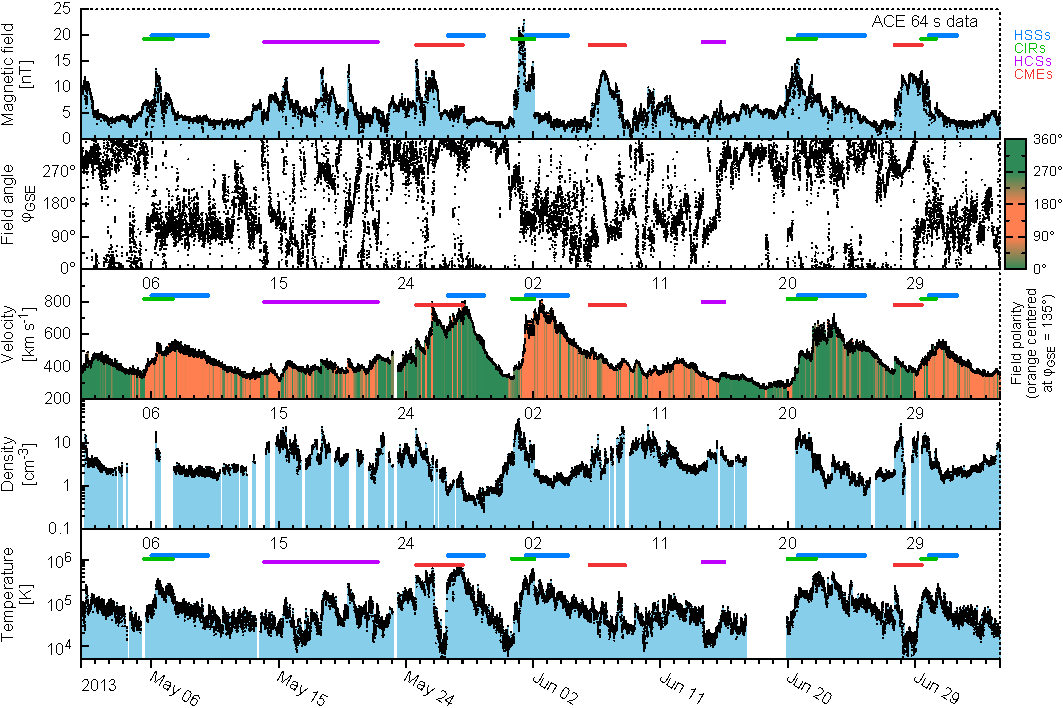
\includegraphics[width=0.9\textwidth]{../figures_of_mine/gnuplots/ACE_64s_v7_thesis_CIRs_2013-5-1_65_plot.pdf}
	\captionoftiny{figure}{\centering Credit: Venzmer, PhD thesis}
\end{frame}
\begin{frame}[plain,c]{Solar wind}{}
	\begin{columns}[c]
	\column{0.5\textwidth}
		
		Measured in-situ throughout the heliosphere:
		\begin{itemize}
			\item Voyager -- heliopause
			\item Ulysses -- high heliolatitudes
			\item Helios -- Mercury
		\end{itemize}
		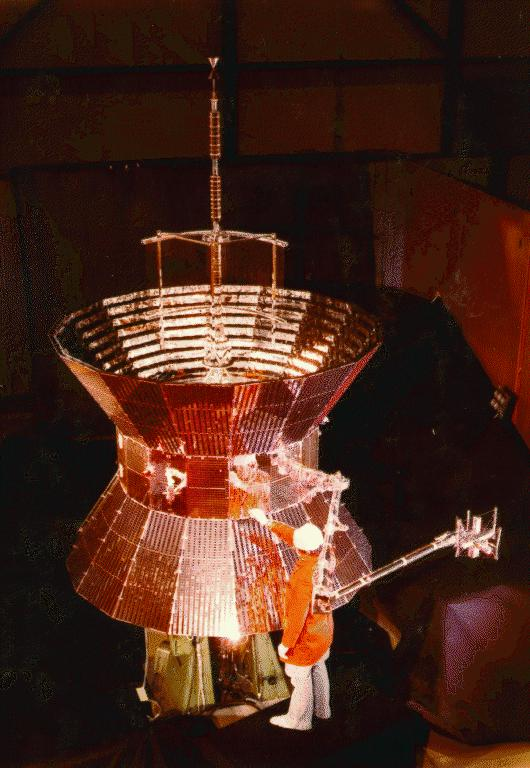
\includegraphics[width=0.1\textwidth]{../figures_of_others/images/helios2.jpg}
		\captionoftiny{figure}{Credit: \href{https://solarsystem.nasa.gov/missions/helios-1/in-depth/}{NASA}}
		
	\column{0.5\textwidth}
		
		image here...

	\end{columns}
\end{frame}

\begin{frame}[plain,c]{Solar wind}{}
	\begin{columns}[c]
	\column{0.65\textwidth}
		
		\hspace*{-17pt}
		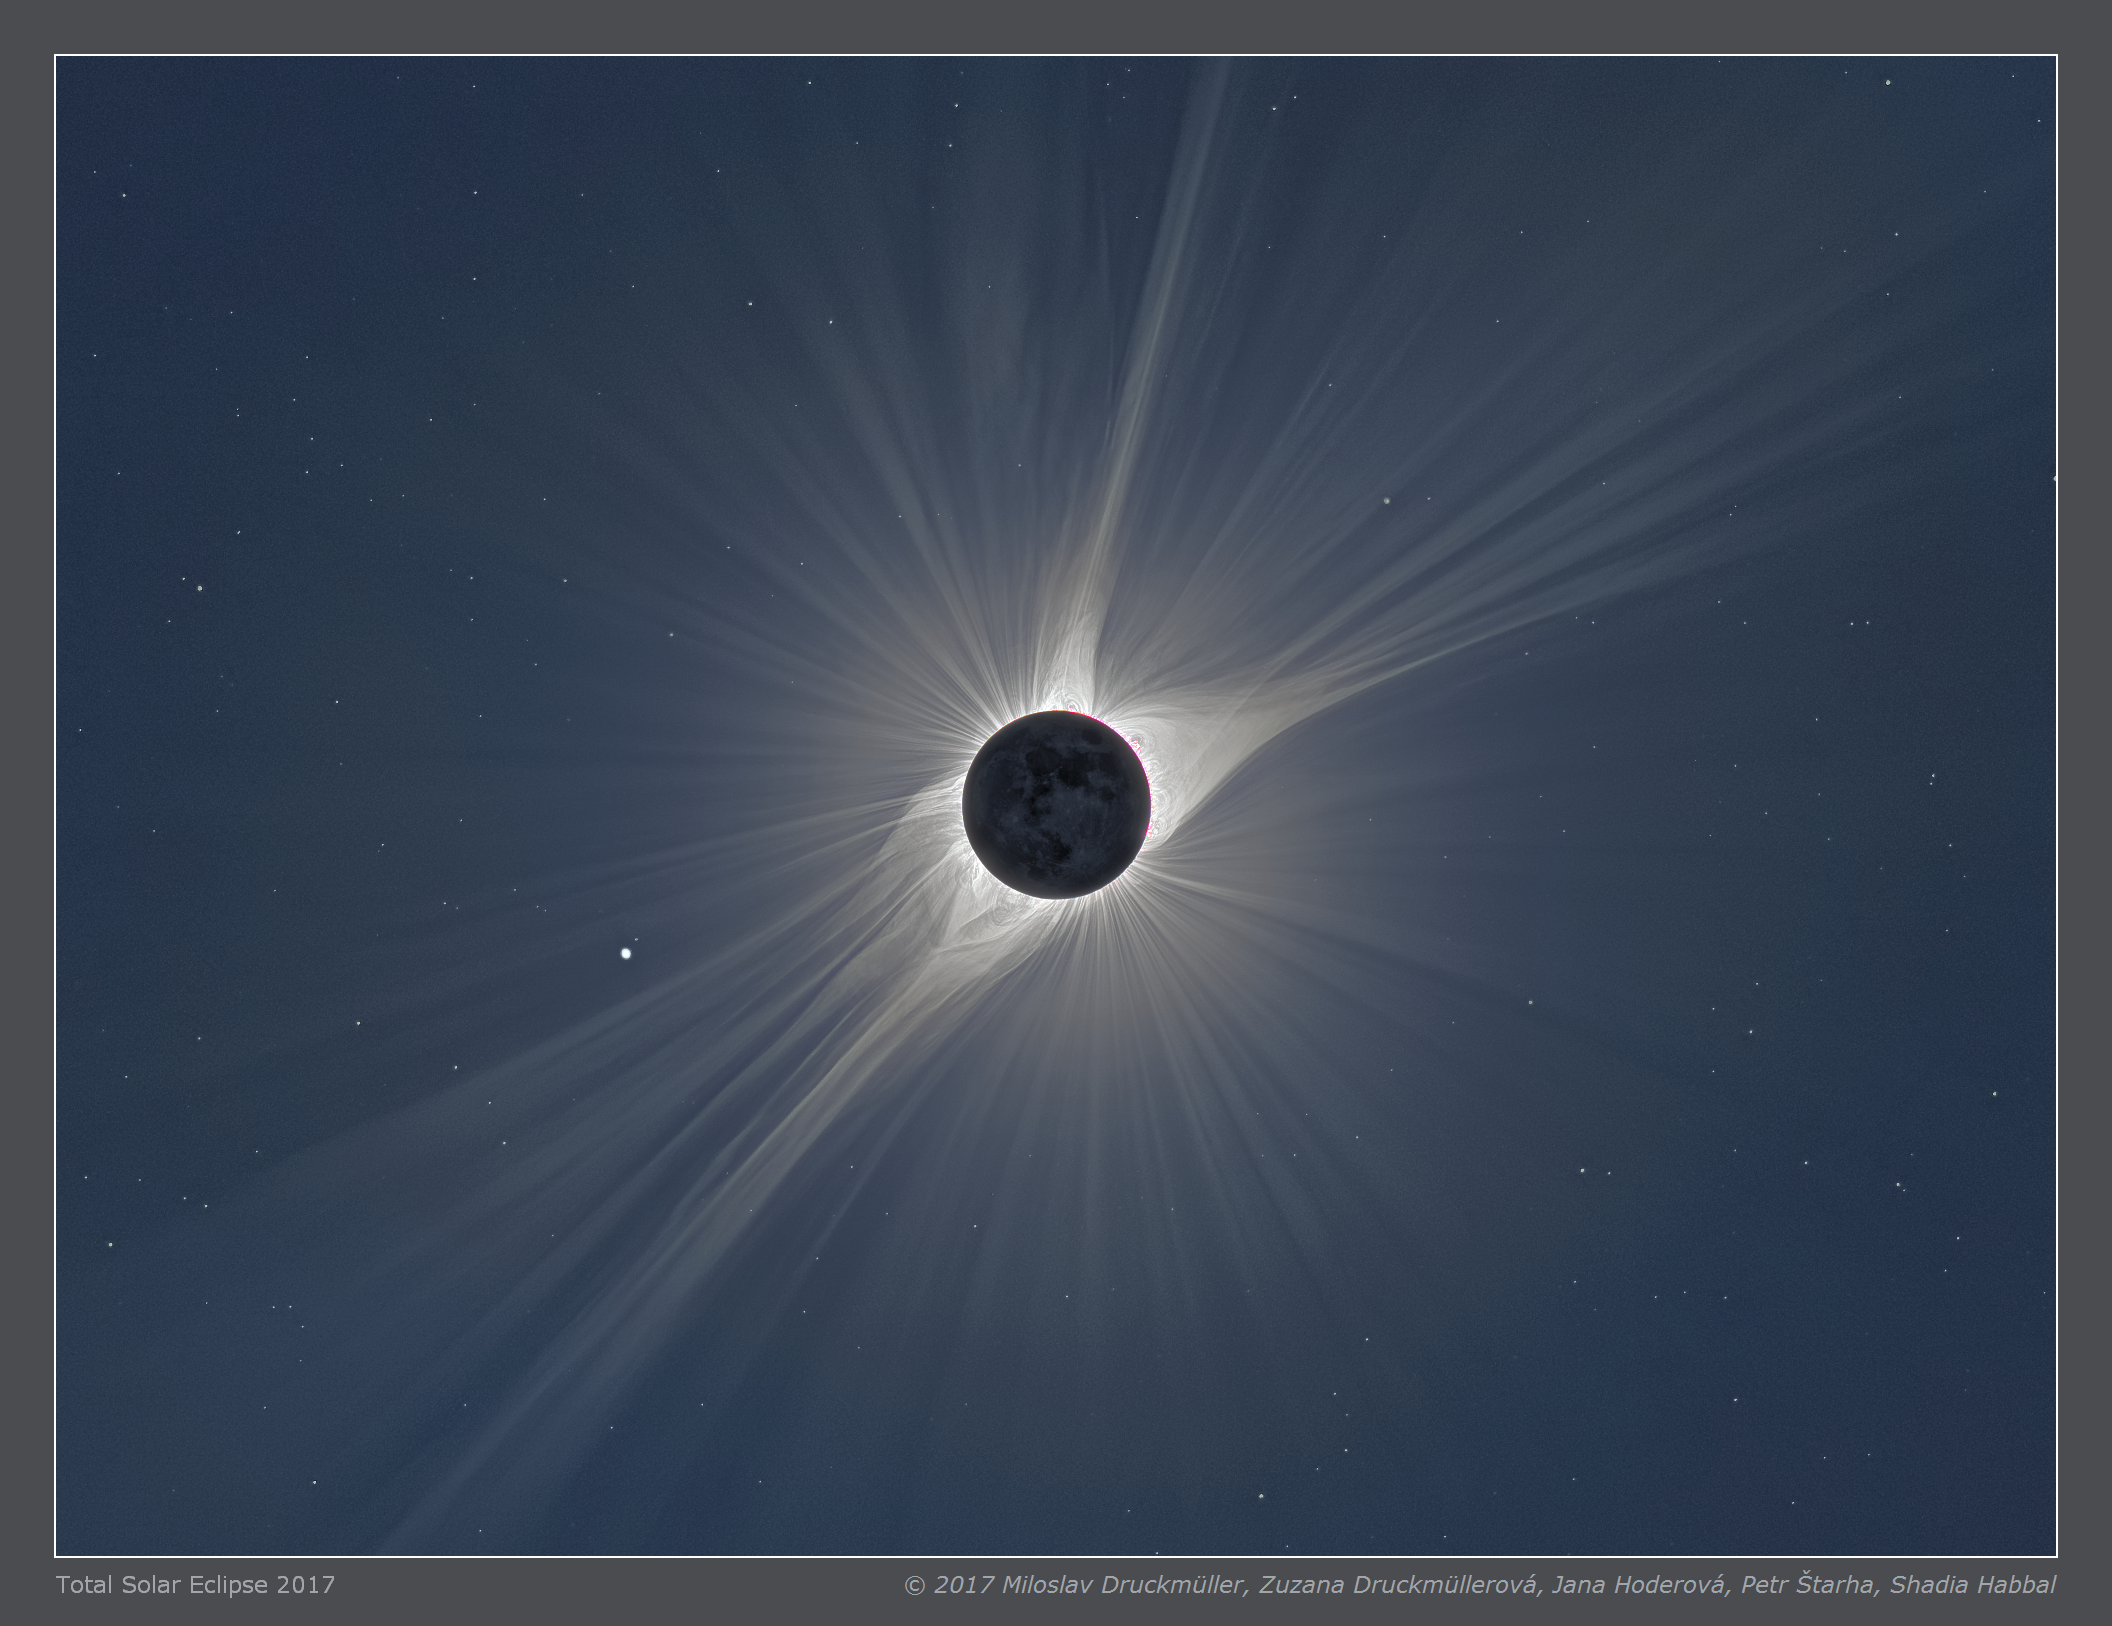
\includegraphics[width=\textwidth]{../talk_figures/TSE_2017_200mm_Whiskey_m-d.png}
		\captionoftiny{figure}{\centering Credit: \href{http://www.zam.fme.vutbr.cz/~druck/Eclipse/}{Miloslav Druckmüller, Zuzana Druckmüllerová, Jana Hoderová, Peter Štarha, Shadia Habbal}, 2017}
		
	\column{0.4\textwidth}
		
		The near-Sun region is of special scientific interest:\\
		\begin{itemize}
			\item Coronal heating
			\item Solar wind acceleration
		\end{itemize}
		
	\end{columns}
\end{frame}
\begin{frame}[plain,c]{Parker Solar Probe}{}
	\begin{columns}[c]
	\column{0.4\textwidth}
		
		\includegraphics[width=\textwidth]{../figures_of_others/images/PSP_fencap2.jpg}
		\captionoftiny{figure}{\centering Credit: \href{http://parkersolarprobe.jhuapl.edu/Multimedia/Images.php}{NASA/Johns Hopkins APL/Ed Whitman}, 2018}

	\column<2->{0.6\textwidth}

		\centering
		\vspace{-4mm}
		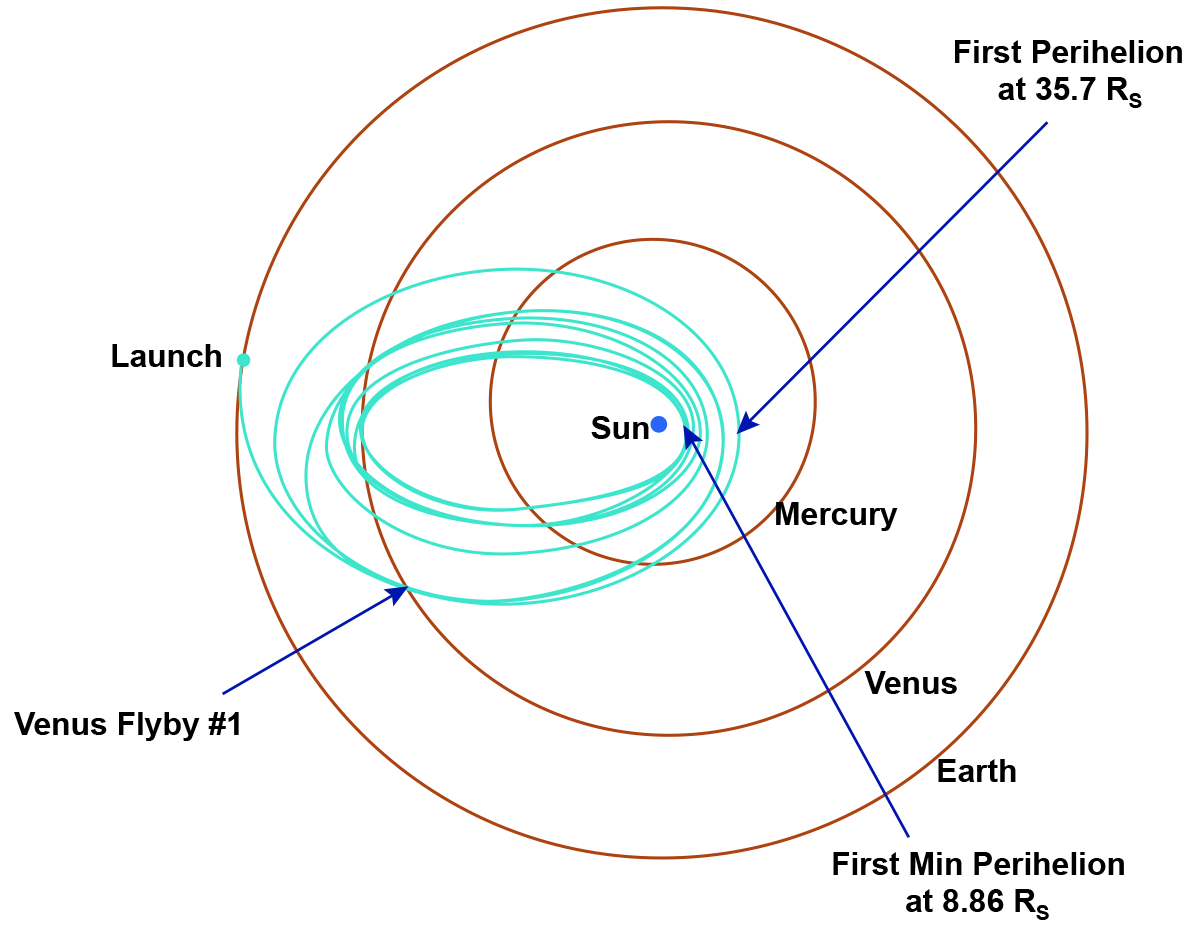
\includegraphics[width=0.75\textwidth]{../figures_of_others/images/PSP_MissionDesign2_negative_crop.png}
		\captionoftiny{figure}{\centering Credit: \href{http://parkersolarprobe.jhuapl.edu/The-Mission/index.php}{NASA/Johns Hopkins APL}, 2018}
		\begin{block}<3>{}
			Launch	\hfill	12 August 2018\\
			1st Venus flyby	\hfill	3 October\\
			Sun-closest spacecraft ever	\hfill	29 October\\
			1st perihelion at 36.7\,\Rs{}	\hfill	6 November\\
			...	\hfill	...\\
			22nd perihelion at 9.86\,\Rs{}	\hfill	24 December 2024
		\end{block}
	\end{columns}
\end{frame}
\begin{frame}[plain,c]{Parker Solar Probe}{}
	\begin{columns}[c]
	\column{\textwidth}
		
% 		\begin{block}{
		PSP mission primary goals \citep{Fox2015}:
			\begin{itemize}
				\item Trace flow of energy that heats and accelerates the corona and solar wind
				\item Determine the structure and dynamics of the plasma and magnetic fields at the sources of the solar wind
				\item Explore the mechanisms that accelerate and transport solar energetic particles
			\end{itemize}
% 		\end{block}
		\vspace{5mm}
		\begin{block}<2>{Scientific instruments}
			\begin{itemize}
				\item FIELDS -- Electromagnetic Fields Investigation
				\item IS\sun{}IS -- Integrated Science Investigation of the Sun
				\item SWEAP -- Solar Wind Electrons Alphas and Protons Investigation
				\item WISPR -- Wide-Field Imager for Solar Probe
			\end{itemize}
		\end{block}

	\end{columns}
\end{frame}


\section{Empirical solar wind model}

\begin{frame}[plain,c]{Solar wind model}{}
	\begin{columns}[c]
	\column{0.5\textwidth}
		
		Aim of this study:
		\begin{itemize}
			\item use existing solar wind data
			\item build empirical solar wind model
			\item extrapolate model to PSP orbit
		\end{itemize}
		\vspace{1cm}
		The major part of this study is published in \citet{Venzmer2018}\\\ 
		
		The article is based on my work performed for the CGAUSS (Coronagraphic German and US SolarProbePlus Survey) project

	\column<2>{0.5\textwidth}
		
		Model concept:\\
		Frequency distributions shifted according to solar activity and solar distance\\
		\begin{block}{Solar wind key parameters}
			\begin{itemize}
				\item Magnetic field strength
				\item Velocity
				\item Density
				\item Temperature
			\end{itemize}
		\end{block}
		
	\end{columns}
\end{frame}

\begin{frame}[plain,c]{PSP distance and solar activity}{}
	\begin{columns}[c]
	\column{0.7\textwidth}
		
		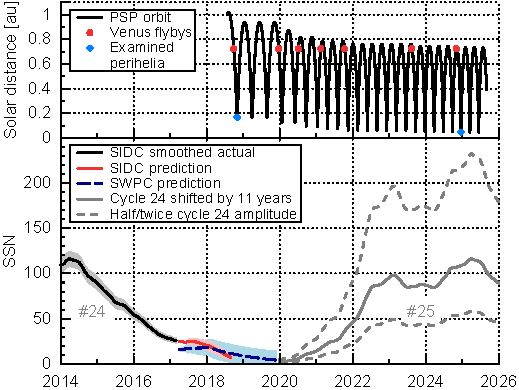
\includegraphics[width=\textwidth]{../figures_paper/SPP_orbit_predicted_SSN_overview_f_plot.pdf}
		\captionoftiny{figure}{\centering Credit: \citet{Venzmer2018}}

	\column<2>{0.3\textwidth}
		
		2018: solar minimum\\
		2024: solar maximum

	\end{columns}
\end{frame}

\begin{frame}[plain,c]{OMNI data set}{}
	\begin{columns}[c]
	\column{\textwidth}
		
		OMNI data set \citep{King2005}\\
		- intercalibrated multi-spacecraft data\\
		- time-shifted to the bow shock of the magnetosphere\\
		- Hourly data since 1963\\
		\centering
		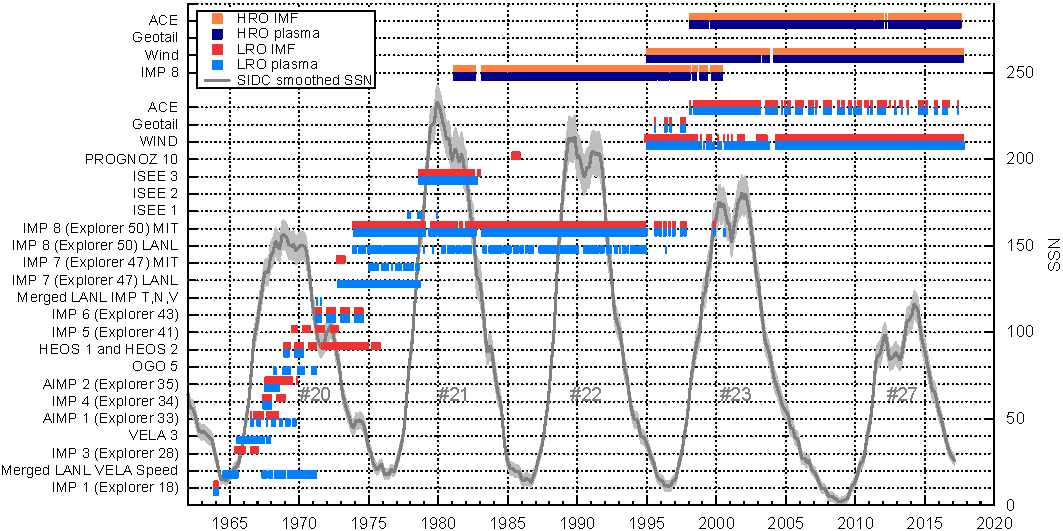
\includegraphics[width=0.9\textwidth]{../figures_of_mine/gnuplots/timeline_OMNI_SC_IDs.pdf}
		\captionoftiny{figure}{\centering Credit: Venzmer, PhD thesis}
		
	\end{columns}
\end{frame}
\begin{frame}[plain,c]{Frequency distributions}{}
	Hourly OMNI data from 1963 to 2016
	\begin{columns}[c]	% [tcb] alignment relative to each column size
	\column{0.7\textwidth}
	
		\hspace*{-21pt}
		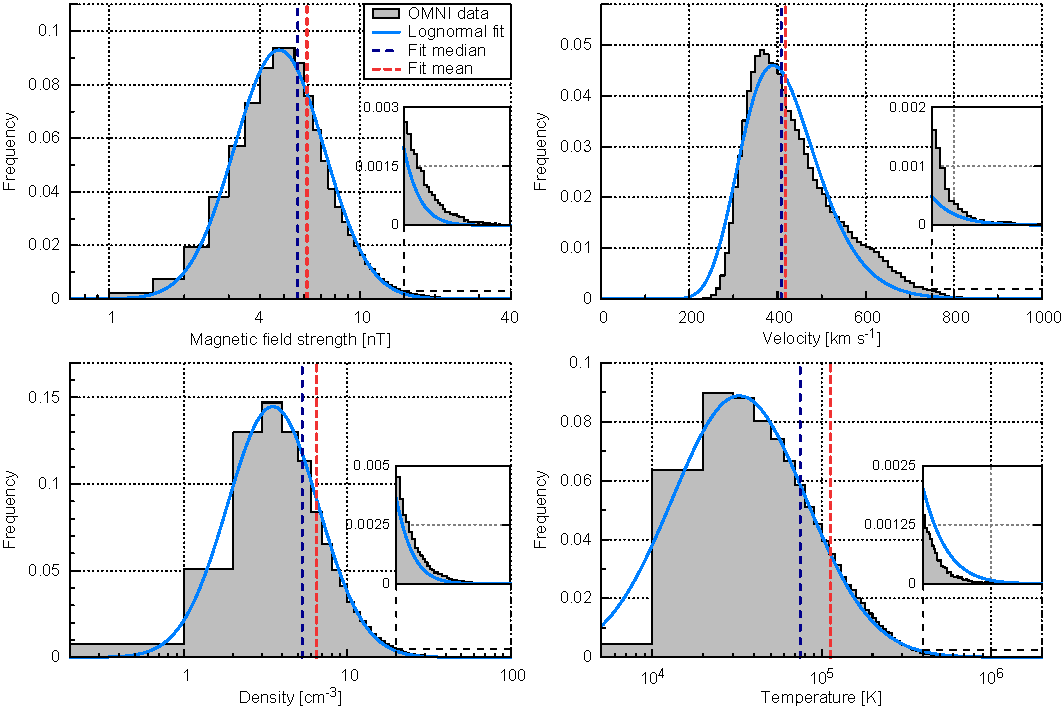
\includegraphics[width=1.1\textwidth]{../figures_paper/histogram_fits_4_a_zoom_paper_pdfplot.pdf}
		\captionoftiny{figure}{\centering Credit: \citet{Venzmer2018}}

	\column<2>{0.3\textwidth}
	
		\hspace*{-10pt}
		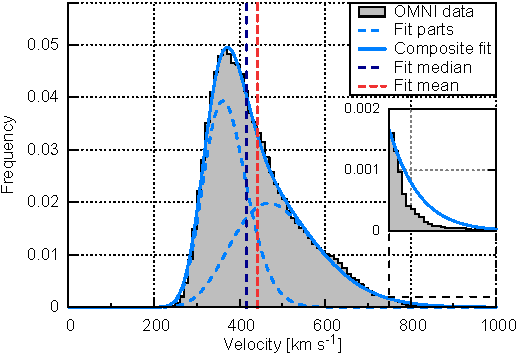
\includegraphics[width=1.2\textwidth]{../figures_paper/histogram_fits_V_a_zoom_dbl_paper_pdfplot.pdf}
		\captionoftiny{figure}{\centering Credit: \citet{Venzmer2018}}

	\end{columns}
	\vspace*{\fill} \hfill \hyperlink{lognormal_distribution}{\beamerskipbutton{}}
\end{frame}
\begin{frame}[plain,c]{Solar activity dependence}{}
	\begin{columns}[c]
	\column{0.5\textwidth}
		
		\hspace*{-10pt}
		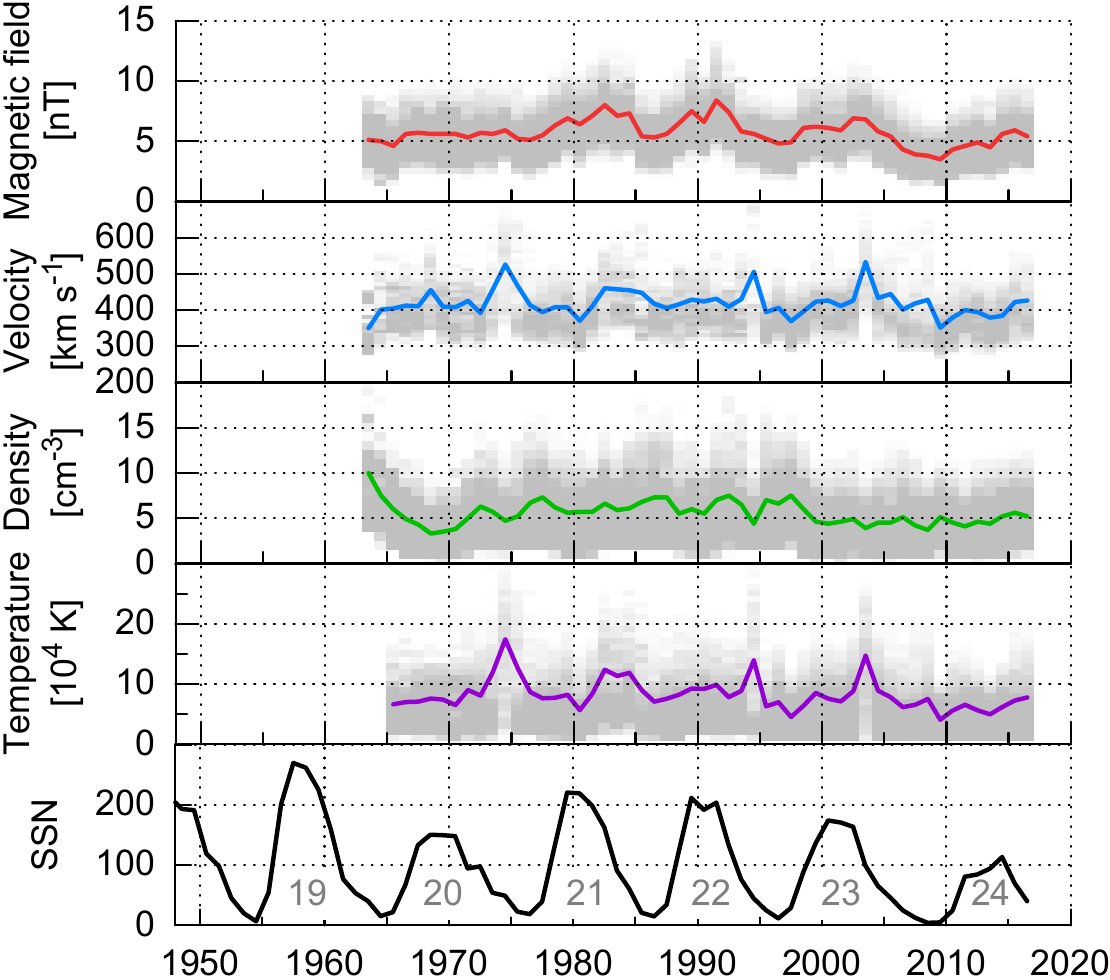
\includegraphics[width=1.1\textwidth]{../talk_figures/SW_SSN_plot.png}
		\captionoftiny{figure}{\centering Credit: \citet{Venzmer2018}}

	\column<2>{0.5\textwidth}
		
		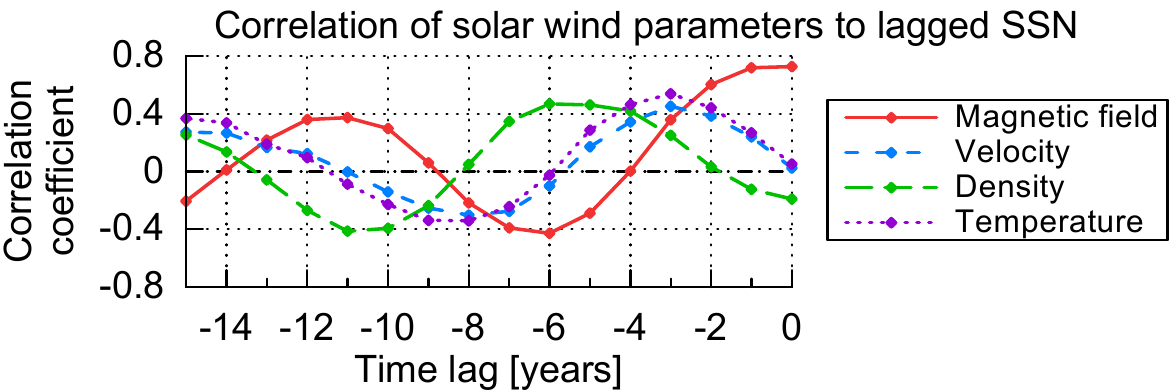
\includegraphics[width=\textwidth]{../talk_figures/SW_SSN_correlation_plot.png}
		\captionoftiny{figure}{\centering Credit: \citet{Venzmer2018}}
		
	\end{columns}
\end{frame}
\begin{frame}[plain,c]{Solar activity dependence}{}
	\begin{columns}[c]
	\column{\textwidth}
		
		\centering
		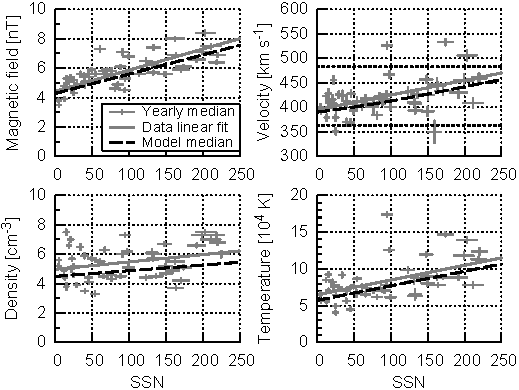
\includegraphics[width=0.7\textwidth]{../figures_paper/OMNI_yearly_BVNTvsSSN_a.pdf}
		\captionoftiny{figure}{\centering Credit: \citet{Venzmer2018}}
		
	\end{columns}
\end{frame}
\begin{frame}[plain,c]{Solar activity dependence}{}
	\centering
	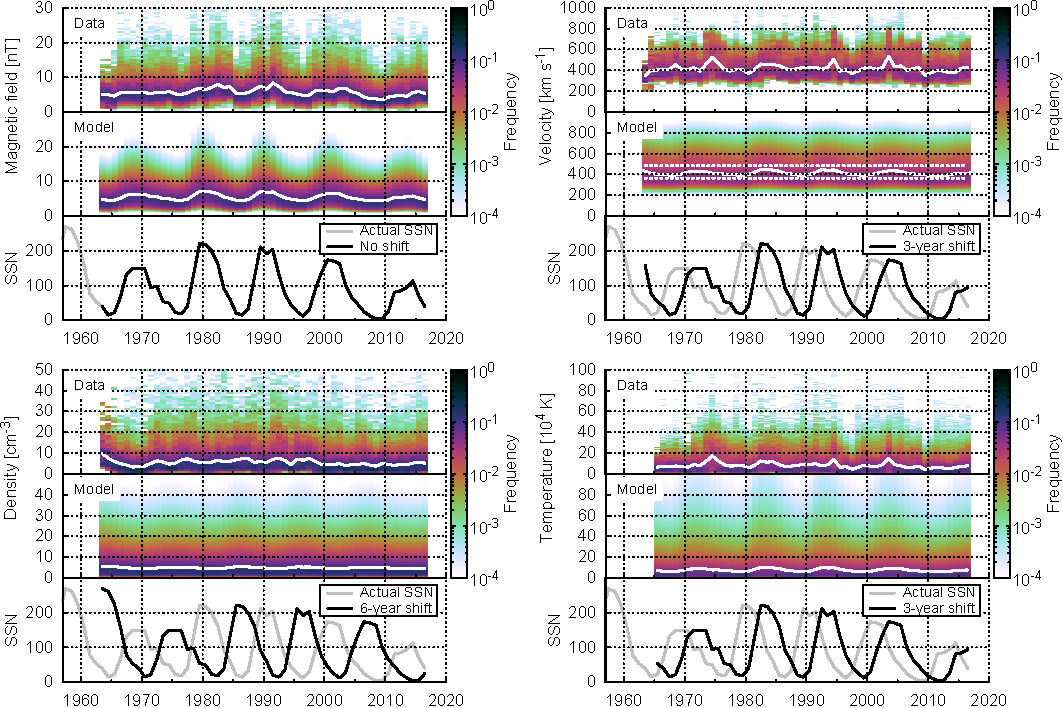
\includegraphics[width=0.9\textwidth]{../figures_paper/OMNI_yearly_BVdblNTSSN_fit_e_plot.pdf}
	\captionoftiny{figure}{\centering Credit: \citet{Venzmer2018}}
\end{frame}
\begin{frame}[plain,c]{Helios data set}{}
	\begin{columns}[c]
	\column{0.5\textwidth}
		
		Helios 1 and Helios 2\\
		\SIrange{0.29}{0.98}{\au}\\
		Hourly data set \citep{Rosenbauer1977}\\
		1974--1981\\\ 
		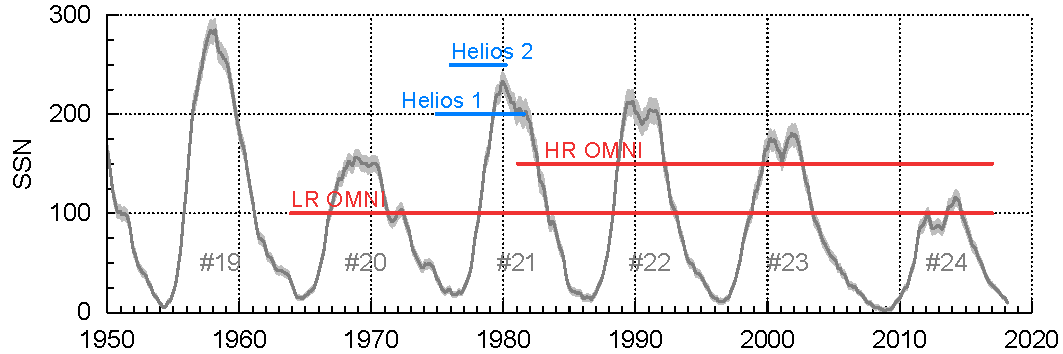
\includegraphics[width=\textwidth]{../talk_figures/timeline_SSN_with_data_and_sc.pdf}
		\captionoftiny{figure}{\centering Credit: Malte Venzmer, 2018}

	\column<2>{0.5\textwidth}

		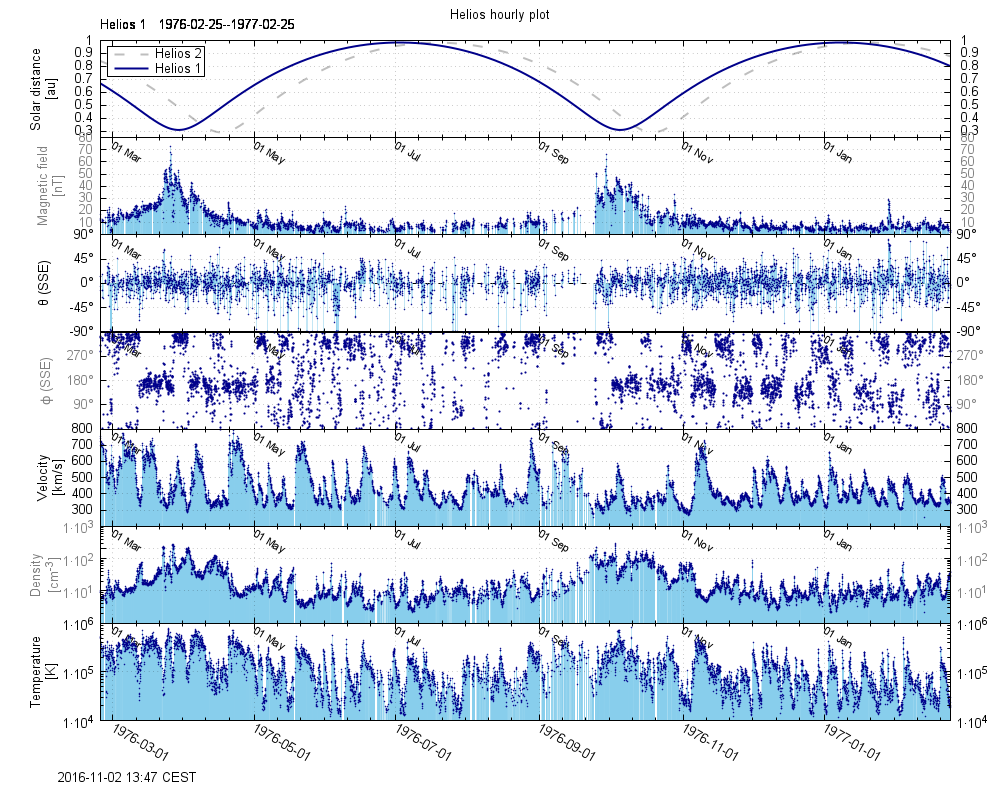
\includegraphics[width=\textwidth]{../talk_figures/hourly_H1_1976-02-25_1977-02-25_plot.png}
		\captionoftiny{figure}{\centering Credit: Malte Venzmer, 2016}
		
	\end{columns}
\end{frame}
\begin{frame}[plain,c]{Solar distance dependence}{}
	\centering
	\includegraphics[width=0.9\textwidth]{../figures_paper/mixed_fit_fixed_4_paper_f_plot.pdf}
	\captionoftiny{figure}{\centering Credit: \citet{Venzmer2018}}
\end{frame}

\begin{frame}[plain,c]{Prediction for PSP orbit}{}
	\begin{columns}[t]	% [tcb] alignment relative to each column size
	\column{0.5\textwidth}
	
		\hspace*{-22pt}
		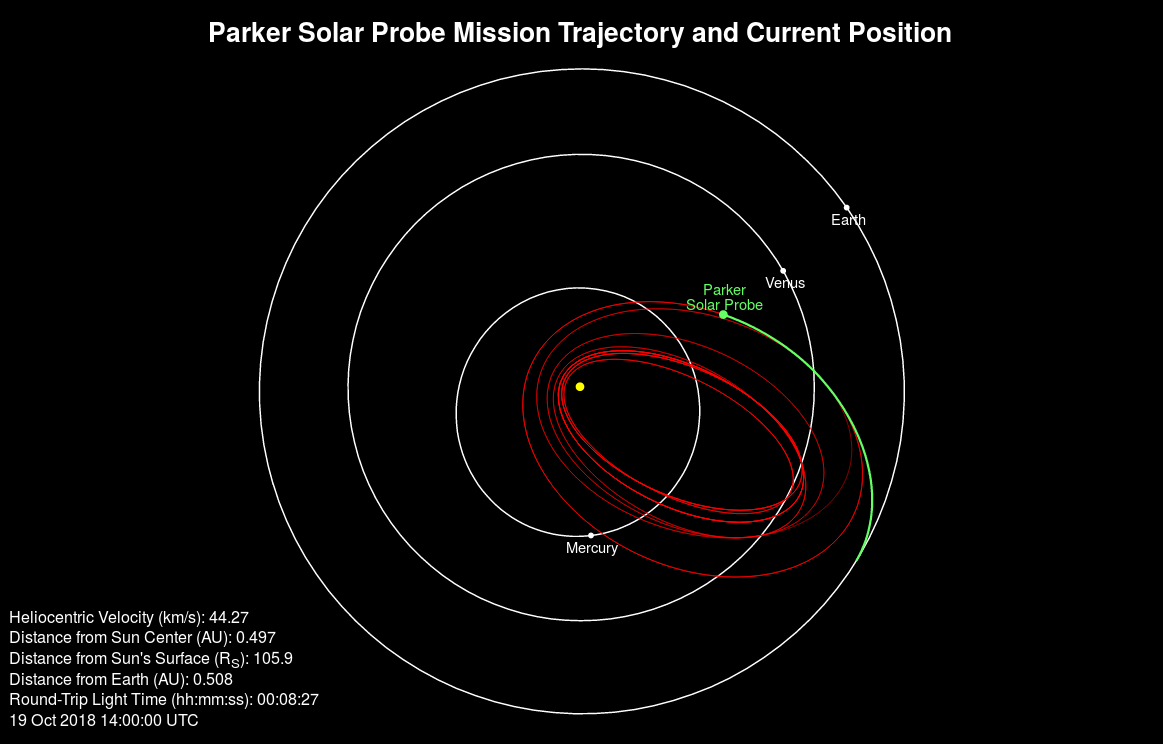
\includegraphics[height=0.9\textwidth]{../talk_figures/psp201810_0400_top.png}
		\captionoftiny{figure}{\centering Credit: \href{http://parkersolarprobe.jhuapl.edu/The-Mission/index.php}{NASA}}

	\column<2>{0.5\textwidth}
	
		\hspace*{-10pt}
		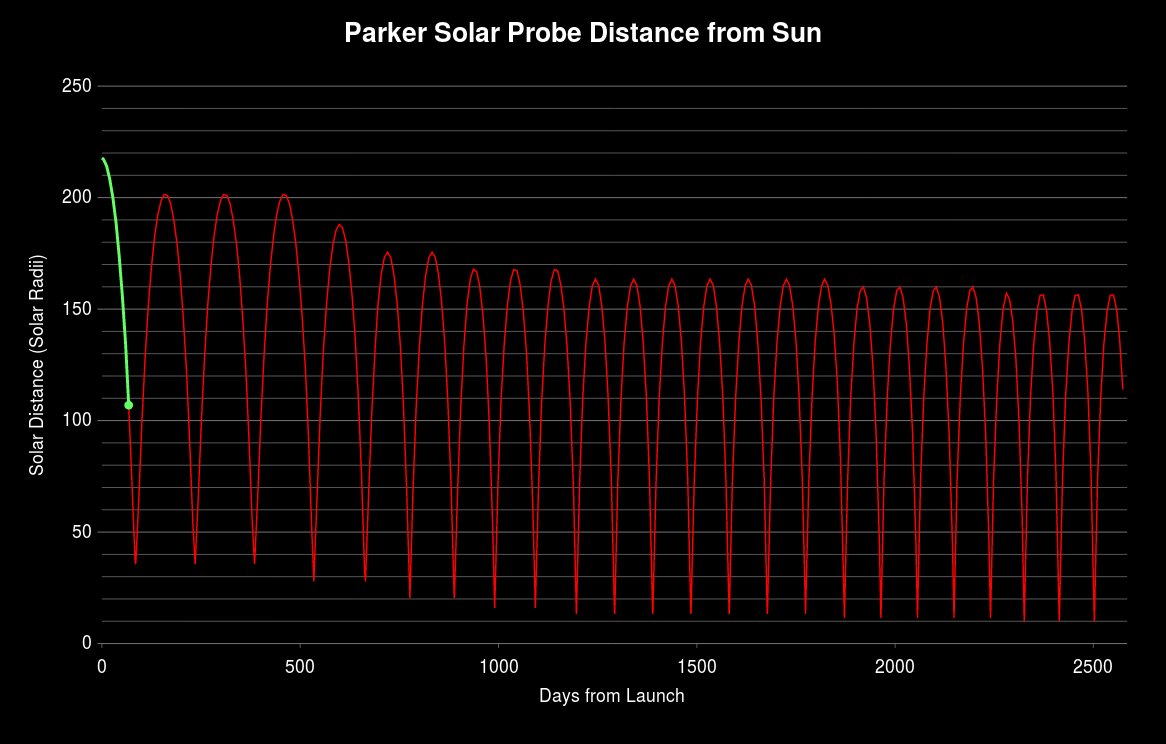
\includegraphics[height=0.9\textwidth]{../talk_figures/psp201810_0400_bottom.png}
		\captionoftiny{figure}{\centering Credit: \href{http://parkersolarprobe.jhuapl.edu/The-Mission/index.php}{NASA}}
		
	\end{columns}
\end{frame}
\begin{frame}[plain,c]{Prediction for PSP orbit}{}
	\begin{columns}[c]
	\column{0.6\textwidth}
		
		\centering
		Perihelion \#1\\\ 
		
		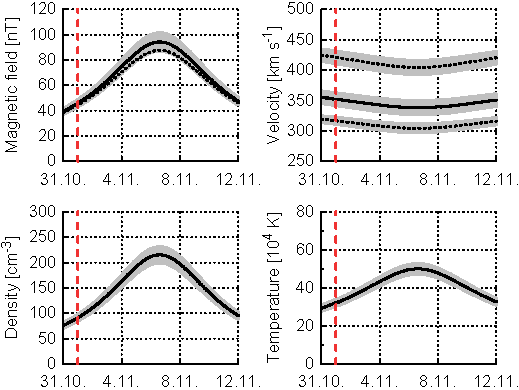
\includegraphics[width=\textwidth]{../talk_figures/SPP_perihelia_prediction_f_defense.pdf}
		\captionoftiny{figure}{\centering Credit: Malte Venzmer, 2018}
		
		November 2018

	\column<2>{0.35\textwidth}
		
		\begin{block}{\centering Predicted values at 36.7~\Rs}
			\begin{align*}
				B &= \SI{94}{\nano\tesla}\\
				v &= \SI{340}{\km\per\s}\\
				n &= \SI{214}{\per\cm\cubed}\\
				T &= \SI{5.03e5}{\kelvin}
			\end{align*}
		\end{block}
	
	\end{columns}
\end{frame}
\begin{frame}[plain,c]{Prediction for PSP orbit}{}
	\begin{columns}[c]
	\column{0.6\textwidth}
		
		\centering
		Perihelion \#22 (first closest)\\\ 
		
		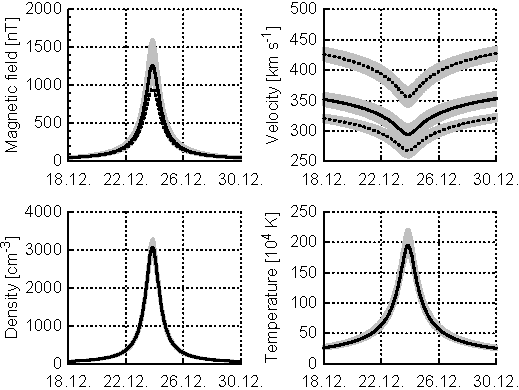
\includegraphics[width=\textwidth]{../talk_figures/SPP_perihelia_prediction_nearest_f_defense.pdf}
		\captionoftiny{figure}{\centering Credit: Malte Venzmer, 2018}
		
		December 2024
		
	\column<2>{0.35\textwidth}
		
		\begin{block}{\centering Predicted values at 9.86\,\Rs}
			\begin{align*}
				B &= \SI{1241}{\nano\tesla}\\
				v &= \SI{290}{\km\per\s}\\
				n &= \SI{2951}{\per\cm\cubed}\\
				T &= \SI{1.93e6}{\kelvin}
			\end{align*}
		\end{block}
		
	\end{columns}
\end{frame}
\begin{frame}[plain,c]{Comparison with other studies}{}
	\begin{columns}[c]
	\column{0.35\textwidth}
		
		\begin{block}{\centering Predicted values at 9.86\,\Rs{}}
			\begin{align*}
				B &= \SI{1241}{\nano\tesla}\\
				v &= \SI{290}{\km\per\s}\\
				n &= \SI{2951}{\per\cm\cubed}\\
				T &= \SI{1.93e6}{\kelvin}
			\end{align*}
		\end{block}

	\column<2->{0.65\textwidth}

		\begin{itemize}[<+->]
			\item Magnetic field values are consistent with theoretical models \citep{Parker1958,Banaszkiewicz1998}
			\item Studies reveal slow wind velocities of \SI{200}{\km\per\s} \citep{Sheeley1997,Wang2000}
			\item Density values agree well with radio burst observations \citep{Leblanc1998}
			\item Near-Sun coronal temperatures yield \SIrange{2}{3}{\mega\kelvin} \citep{Billings1959,Liebenberg1975}
		\end{itemize}
	\end{columns}
	
	\vspace{5mm}
	
	\begin{columns}[c]
	\column<+->{\textwidth}
	
	Remote observations show the limits of the extrapolation

	\begin{block}{Velocity and temperature are overestimated}
		\centering $\Rightarrow$ Solar wind is still being heated and accelerated up to 20\,\Rs{}
	\end{block}
	
	\end{columns}
\end{frame}


\section{Summary}

\begin{frame}[c]{Summary}{}
	
	I derived an empirical solar wind model for the inner heliosphere that considers solar activity and solar distance
	\begin{itemize}%[<+->]
		\item Extrapolation of the model to the near-Sun environment for the PSP orbit
		\item Solar wind prediction for PSP's first and first closest perihelia
	\end{itemize}
	
\end{frame}
\begin{frame}[plain,c]{Outlook}{}
	\begin{columns}[c]
	\column{\textwidth}
		
		\begin{itemize}
			\item Possible modifications to model (e.g., flux conservation)
			\item Refine model with additional solar wind data from Mercury probes and the upcoming Solar Orbiter
			\item Parker Solar Probe measurements can be used to validate the extrapolations
		\end{itemize}
		
		\vspace{1cm}
		
		\action<2>{\centering\LARGE\color{blue} Thank you!}
		
	\end{columns}
\end{frame}

\begin{frame}[t,allowframebreaks]{References}
	\tiny
	\begin{thebibliography}{10}
	
		\beamertemplatebookbibitems
		
		\beamertemplatearticlebibitems
		
		
\bibitem[{{Bothmer} \& {Schwenn}(1998)}]{Bothmer1998}
	{Bothmer}, V. \& {Schwenn}, R. 1998, \emph{{The structure and origin of magnetic clouds in the solar
	wind}}, Annales Geophysicae, 16, 1,
	\href{http://dx.doi.org/10.1007/s00585-997-0001-x}{[DOI]},
	\href{http://adsabs.harvard.edu/abs/1998AnGeo..16....1B}{[ADS]}.

\bibitem[{{Cranmer} \& {van Ballegooijen}(2005)}]{Cranmer2005}
	{Cranmer}, S.~R. \& {van Ballegooijen}, A.~A. 2005, \emph{{On the Generation,
	Propagation, and Reflection of Alfv{\'e}n Waves from the Solar Photosphere to
	the Distant Heliosphere}}, \apjs, 156, 265,
	\href{http://dx.doi.org/10.1086/426507}{[DOI]},
	\href{http://adsabs.harvard.edu/abs/2005ApJS..156..265C}{[ADS]}.

\bibitem[{Davies(1990)}]{Davies1990}
	Davies, K. 1990, \emph{Ionospheric Radio} (Institution of Engineering and
	Technology),
	\href{http://digital-library.theiet.org/content/books/ew/pbew031e}{[link]},
	\href{http://dx.doi.org/10.1049/PBEW031E}{[DOI]}.

\bibitem[{{Hathaway}(2015)}]{Hathaway2015}
	{Hathaway}, D.~H. 2015, \emph{{The Solar Cycle}}, Living Reviews in Solar
	Physics, 12, 4, \href{http://dx.doi.org/10.1007/lrsp-2015-4}{[DOI]},
	\href{http://adsabs.harvard.edu/abs/2015LRSP...12....4H}{[ADS]}.

\bibitem[{{Hughes}(1995)}]{Hughes1995}
	{Hughes}, W.~J. 1995, \emph{{Chapter 9: The magnetopause, magnetotail, and
	magnetic reconnection}}, ed. M.~Kivelson \& C.~Russell, Introduction to Space
	Physics (Cambridge University Press, Cambridge), 227--287,
	\href{http://adsabs.harvard.edu/abs/1995isp..book.....K}{[ADS]}.

\bibitem[{{Marubashi} \& {Lepping}(2007)}]{Marubashi2007}
	{Marubashi}, K. \& {Lepping}, R.~P. 2007, \emph{{Long-duration magnetic clouds:
	a comparison of analyses using torus- and cylinder-shaped flux rope models}},
	Annales Geophysicae, 25, 2453,
	\href{http://dx.doi.org/10.5194/angeo-25-2453-2007}{[DOI]},
	\href{http://adsabs.harvard.edu/abs/2007AnGeo..25.2453M}{[ADS]}.
	
\bibitem[{{McComas} {et~al.}(2008{\natexlab{a}}){McComas}, {Ebert}, {Elliott},
	{Goldstein}, {Gosling}, {Schwadron}, \& {Skoug}}]{McComas200809}
	{McComas}, D.~J., {Ebert}, R.~W., {Elliott}, H.~A. {et~al.} 2008{\natexlab{a}},
	\emph{{Weaker solar wind from the polar coronal holes and the whole Sun}},
	\grl, 35, L18103, \href{http://dx.doi.org/10.1029/2008GL034896}{[DOI]},
	\href{http://adsabs.harvard.edu/abs/2008GeoRL..3518103M}{[ADS]}.

\bibitem[{{Owens} \& {Forsyth}(2013)}]{Owens2013}
	{Owens}, M.~J. \& {Forsyth}, R.~J. 2013, \emph{{The Heliospheric Magnetic
	Field}}, Living Reviews in Solar Physics, 10, 5,
	\href{http://dx.doi.org/10.12942/lrsp-2013-5}{[DOI]},
	\href{http://adsabs.harvard.edu/abs/2013LRSP...10....5O}{[ADS]}.

\bibitem[{{Parker}(1958)}]{Parker1958}
	{Parker}, E.~N. 1958, \emph{{Dynamics of the Interplanetary Gas and Magnetic Fields.}}, \apj, 128, 664, \href{http://dx.doi.org/10.1086/146579}{[DOI]}, \href{http://adsabs.harvard.edu/abs/1958ApJ...128..664P}{[ADS]}.

\bibitem[{{Pizzo}(1991)}]{Pizzo1991}
	{Pizzo}, V.~J. 1991, \emph{{The evolution of corotating stream fronts near the
	ecliptic plane in the inner solar system. II - Three-dimensional
	tilted-dipole fronts}}, \jgr, 96, 5405,
	\href{http://dx.doi.org/10.1029/91JA00155}{[DOI]},
	\href{http://adsabs.harvard.edu/abs/1991JGR....96.5405P}{[ADS]}.
	
\bibitem[{{Schatten} {et~al.}(1969){Schatten}, {Wilcox}, \&
	{Ness}}]{Schatten1969}
	{Schatten}, K.~H., {Wilcox}, J.~M. \& {Ness}, N.~F. 1969, \emph{{A model of
	interplanetary and coronal magnetic fields}}, \solphys, 6, 442,
	\href{http://dx.doi.org/10.1007/BF00146478}{[DOI]},
	\href{http://adsabs.harvard.edu/abs/1969SoPh....6..442S}{[ADS]}.

\bibitem[{{Venzmer} \& {Bothmer}(2018)}]{Venzmer2018}
	{Venzmer}, M.~S. \& {Bothmer}, V. 2018, \emph{{Solar-wind predictions for the
	Parker Solar Probe orbit. Near-Sun extrapolations derived from an empirical
	solar-wind model based on Helios and OMNI observations}}, \aap, 611, A36,
	\href{http://dx.doi.org/10.1051/0004-6361/201731831}{[DOI]},
	\href{http://adsabs.harvard.edu/abs/2018A\%26A...611A..36V}{[ADS]}.



	\end{thebibliography}
\end{frame}
% {\usebackgroundtemplate{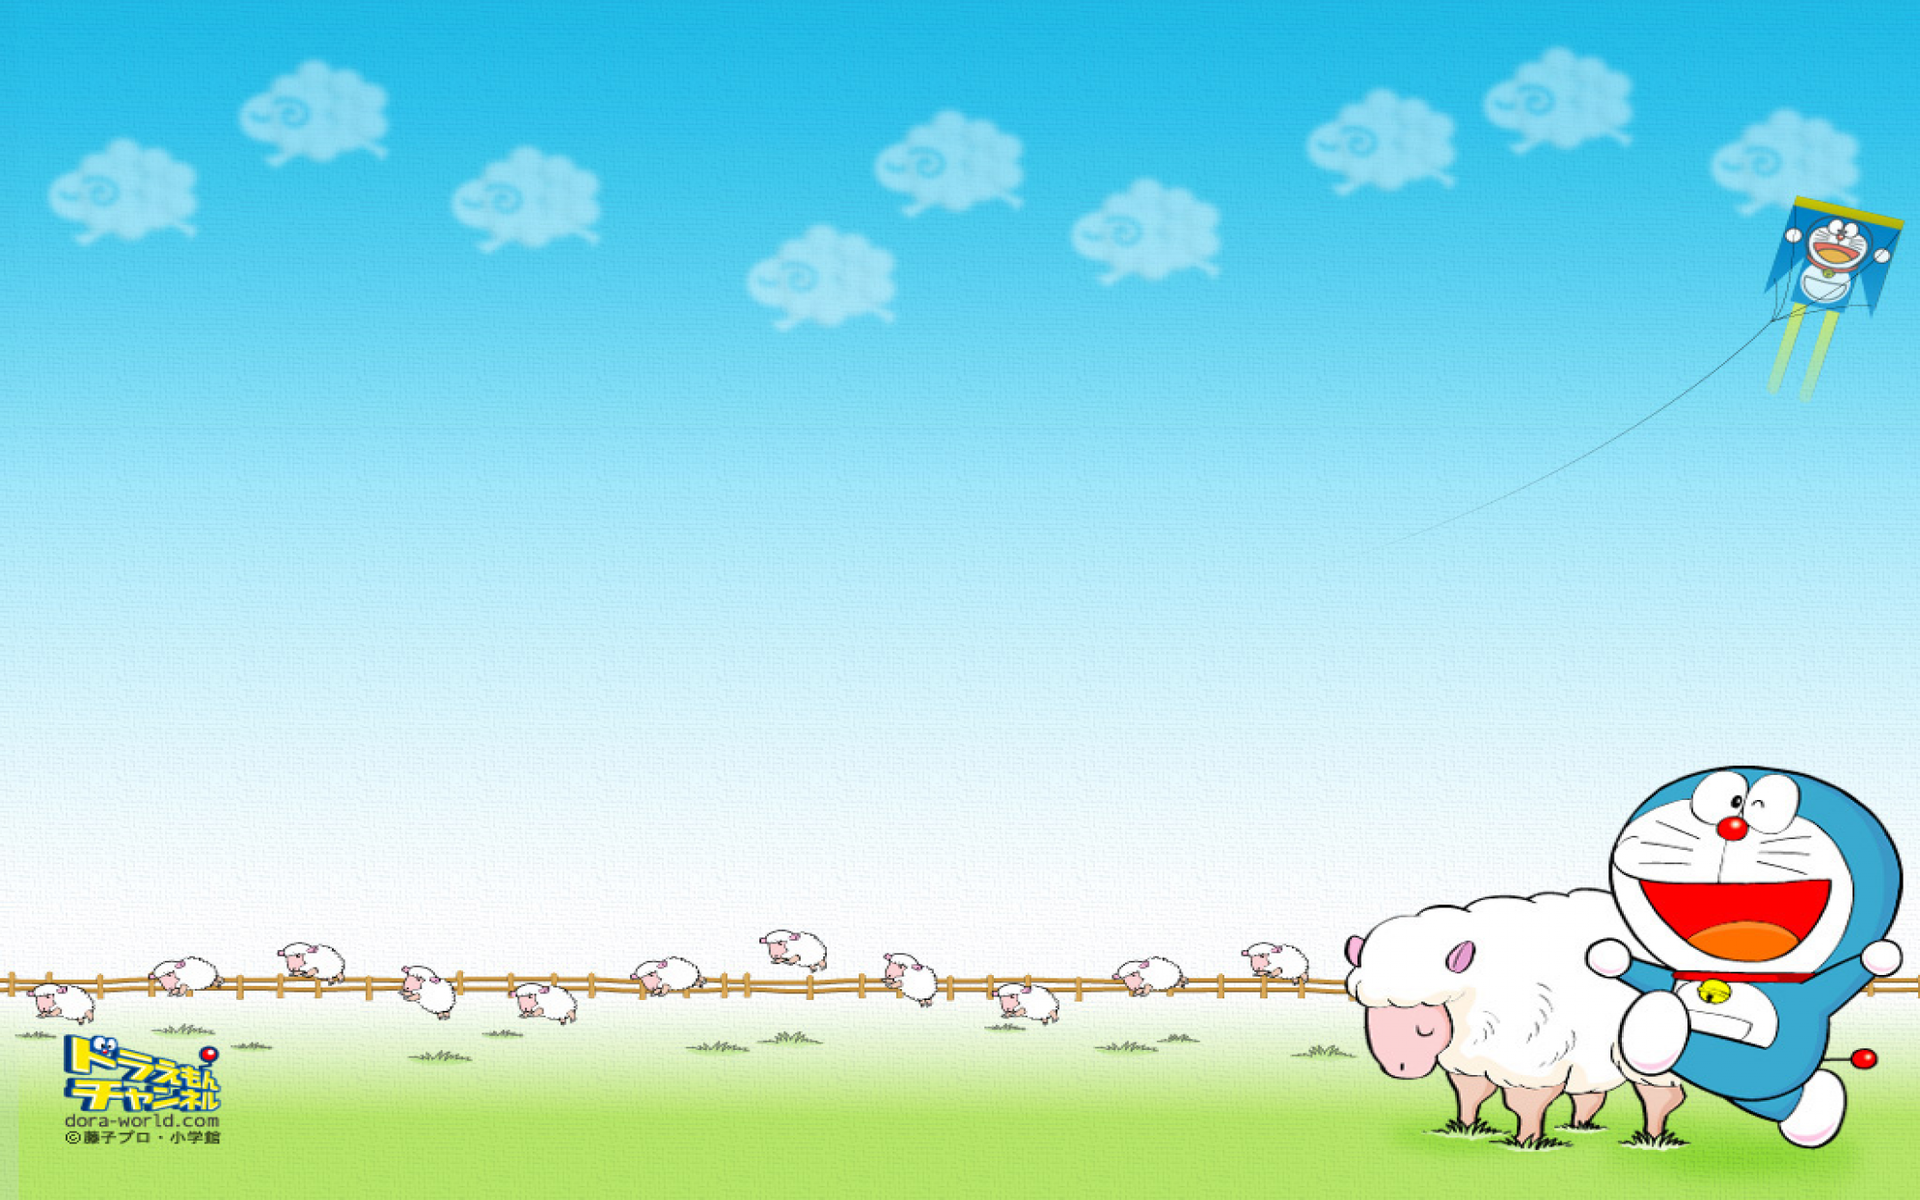
\includegraphics[width=\paperwidth]{../talk_figures/doraemon-und-schaf_1920x1200_48191.png}}
% \begin{frame}[c,plain]{}{}
% 	\centering
% 	\Large Thank you!
% \end{frame}
% }


\appendix


\section{Backup slides}

\subsection{Solar wind}

\begin{frame}[c,label=butterfly]{Solar activity}{Magnetic butterfly diagram}
% 	\hypertarget{butterfly}{\beamerbutton{I'm on this slide}}
	
	\centering
	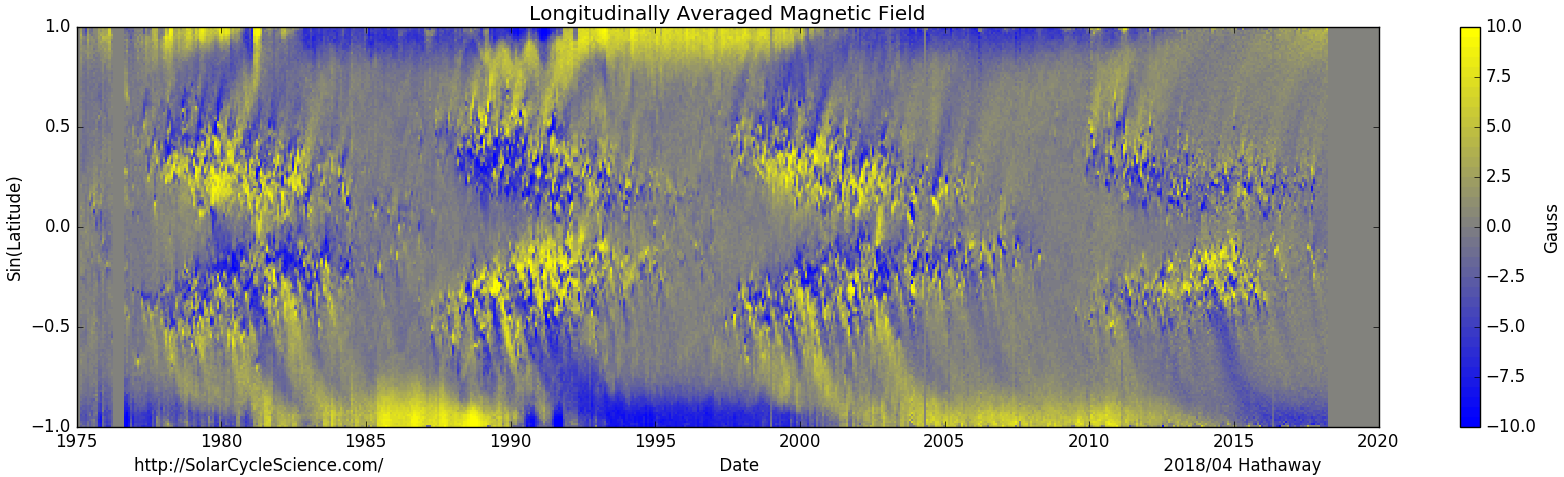
\includegraphics[width=\textwidth]{../figures_of_others/images/Hathaway_magbfly_201804_cropped.png}
	\captionoftiny{figure}{\centering Courtesy of David~Hathaway, \href{http://solarcyclescience.com/solarcycle.html}{Solar Cycle Science}, 2018, updated version of {\citet[Fig.~17]{Hathaway2015}}}
\end{frame}
\begin{frame}[plain,c]{Solar wind}{}
	\centering
	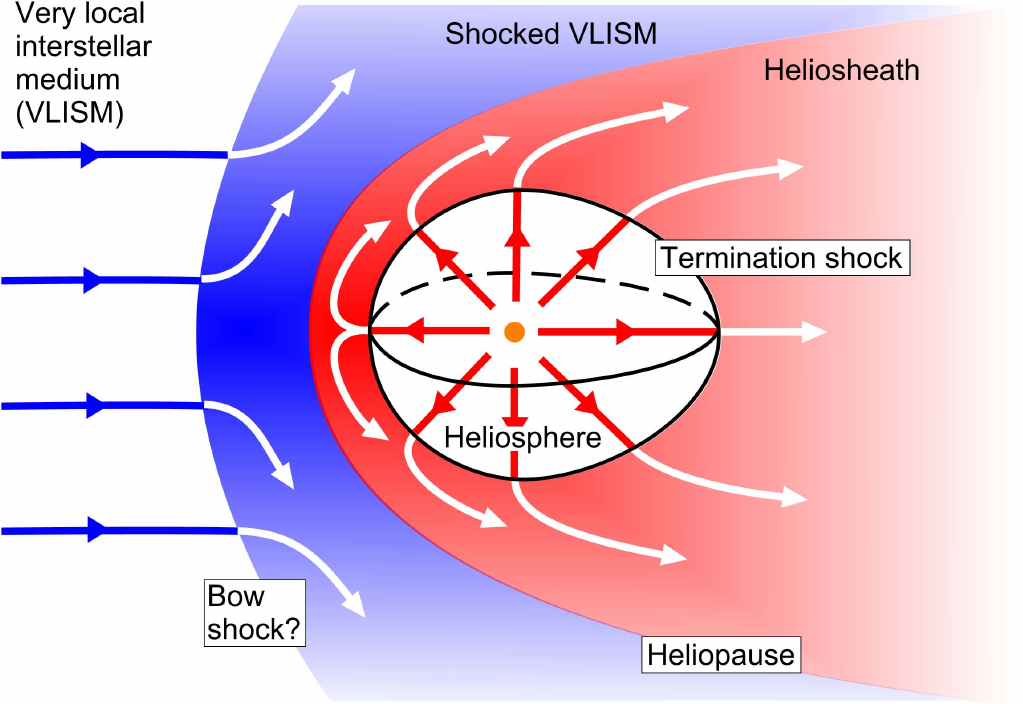
\includegraphics[width=0.8\textwidth]{../figures_of_others/images/Owens2013_Heliosphere_screenshot.png}
	\captionoftiny{figure}{\centering Credit: {\citet[Fig.~9]{Owens2013}}}
\end{frame}
\begin{frame}[plain,c]{Solar wind}{}
	\centering
	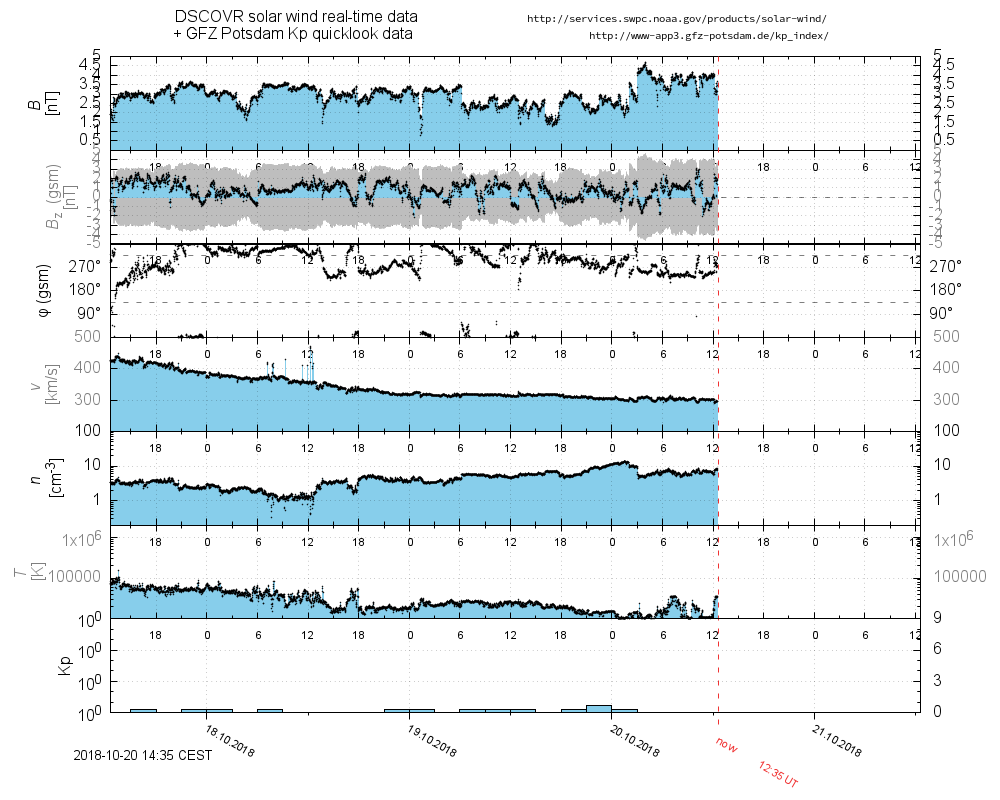
\includegraphics[width=0.7\textwidth]{../talk_figures/ace_realtime_ap_plot.png}
\end{frame}

\begin{frame}[plain,c]{Solar magnetic field}{}
	\centering
	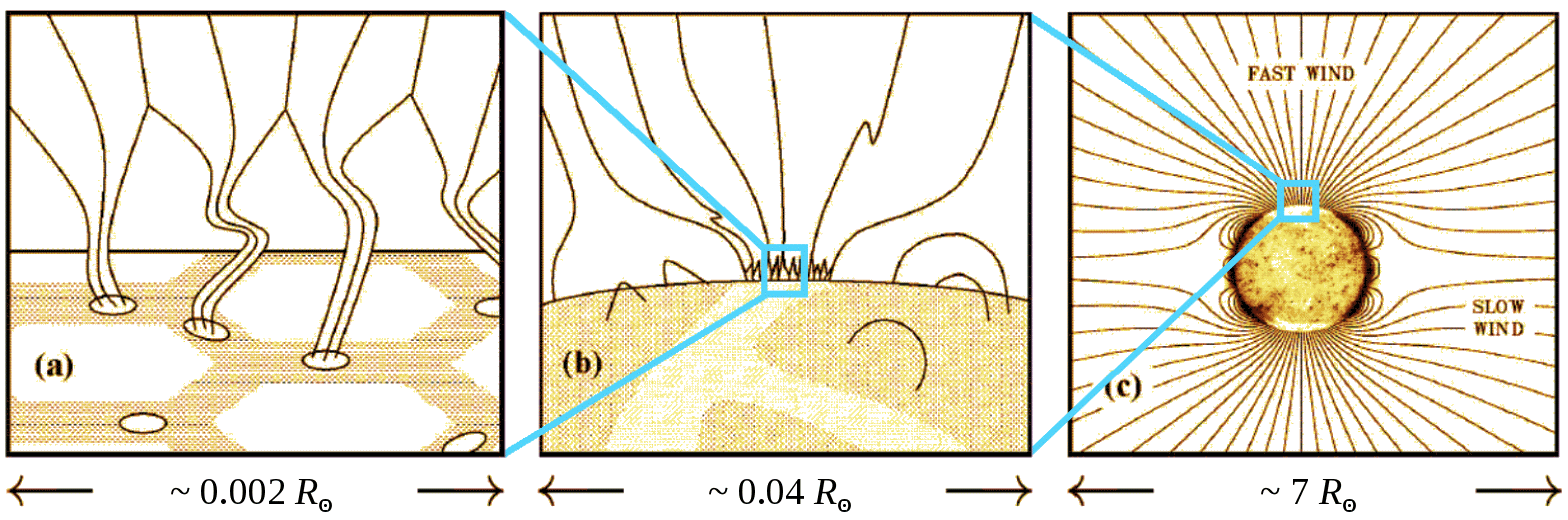
\includegraphics[width=0.8\textwidth]{../figures_of_others/images/Cranmer2005_fig1_color.png}
	\captionoftiny{figure}{Courtesy of S. R. Cranmer}
\end{frame}
\begin{frame}[plain,c]{Solar magnetic field}{}
	\begin{columns}[c]
	\column{\textwidth}

	\centering
	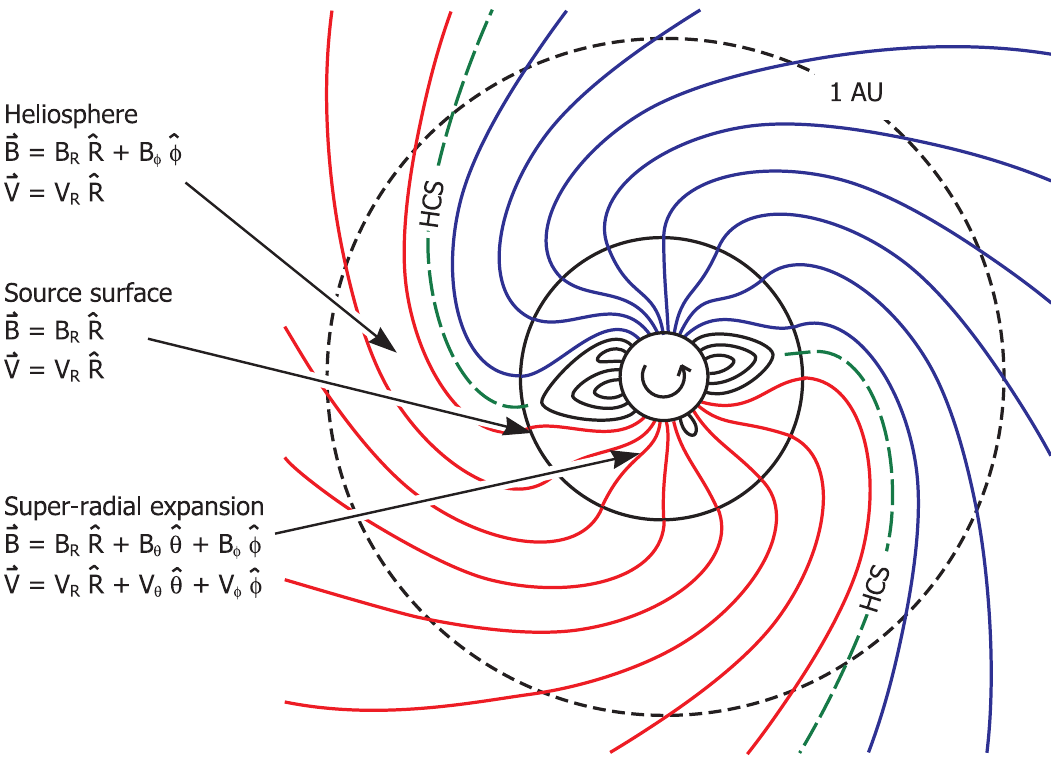
\includegraphics[width=0.7\textwidth]{../figures_of_others/images/Owens2013_PFSS_Sectors_screenshot.png}
	\captionoftiny{figure}{\centering Credit: {\citet[Fig.~1]{Owens2013}}, adapted from {\citet[Fig.~1]{Schatten1969}}}
	
	\end{columns}
\end{frame}
\begin{frame}[plain,c]{Slow and fast solar wind}{}
	\begin{columns}[c]
	\column{0.5\textwidth}

	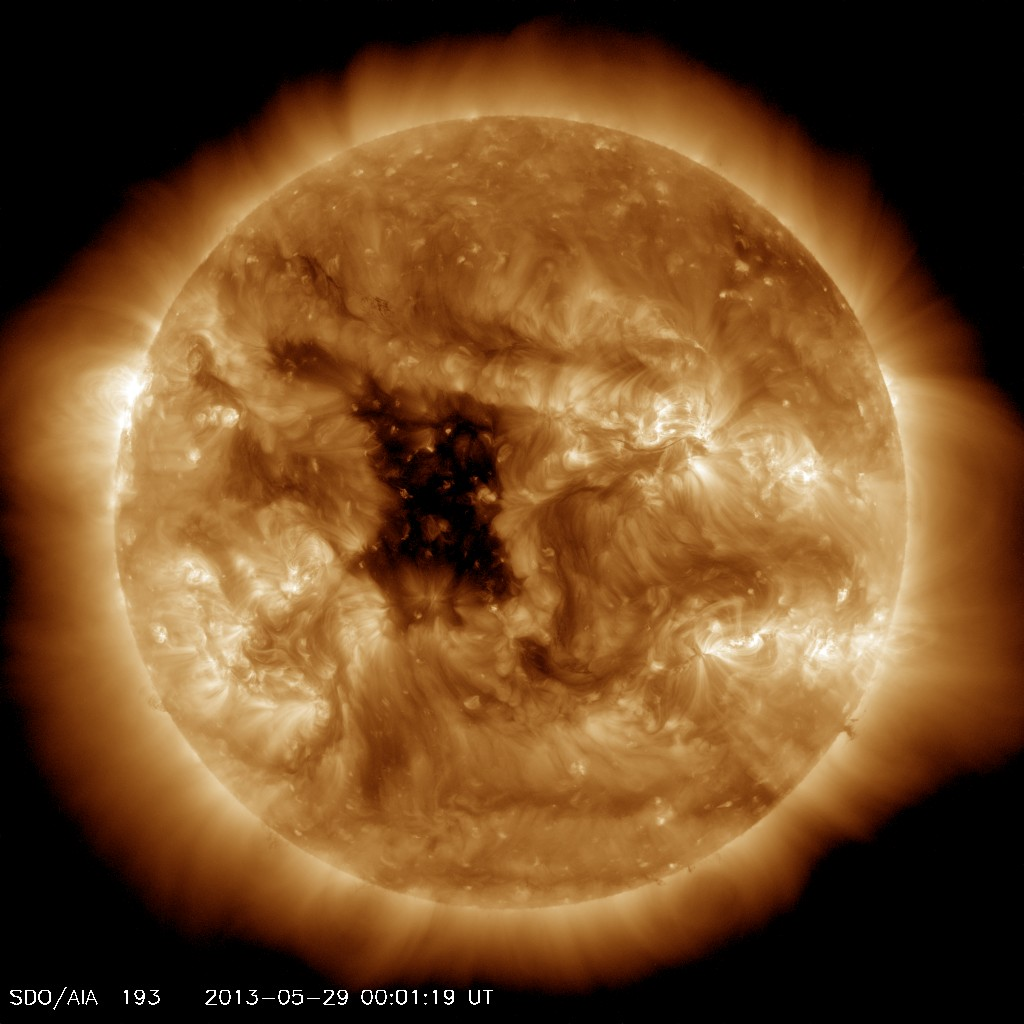
\includegraphics[width=\textwidth]{../figures_of_others/images/20130529_000119_1024_0193.jpg}
	\captionoftiny{figure}{\centering Credit: NASA/SDO and the AIA, EVE and HMI science teams}
	
	\column{0.5\textwidth}
	
	\end{columns}
\end{frame}
\begin{frame}[plain,c]{Slow and fast solar wind}{}
	\centering
	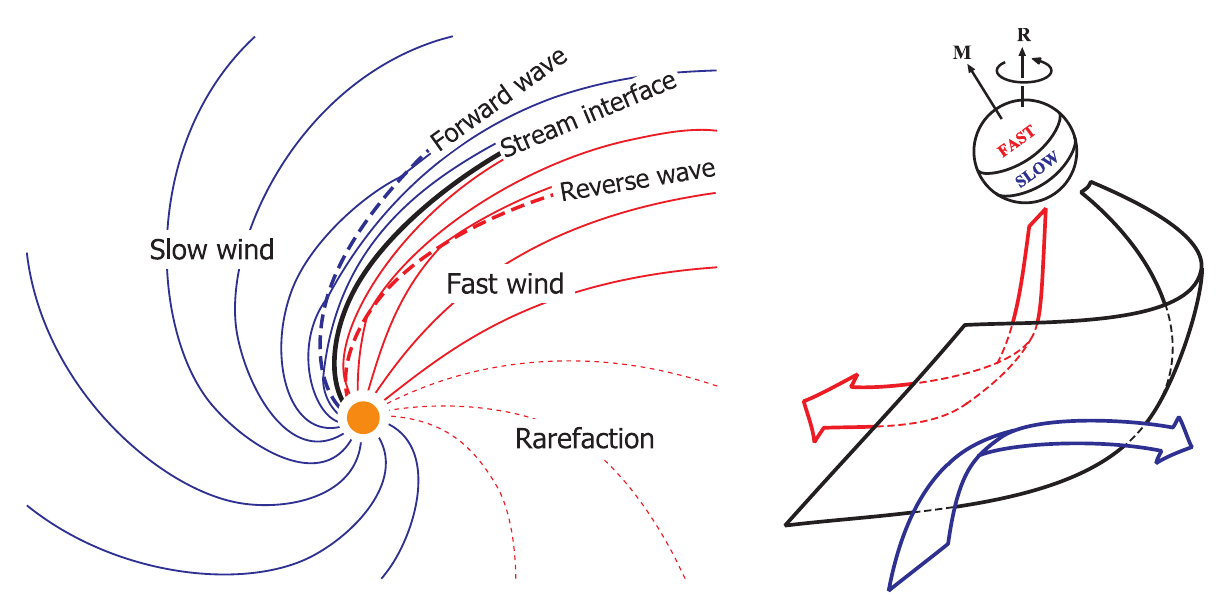
\includegraphics[width=0.9\textwidth]{../figures_of_others/images/Owens2013_CIR_2panel_screenshot.png}
	\captionoftiny{figure}{\centering Credit: {\citet[Fig.~7]{Owens2013}}; right panel adapted from {\citet[Fig.~2]{Pizzo1991}}}
\end{frame}

\begin{frame}[plain,c]{Solar activity}{}
	\centering
	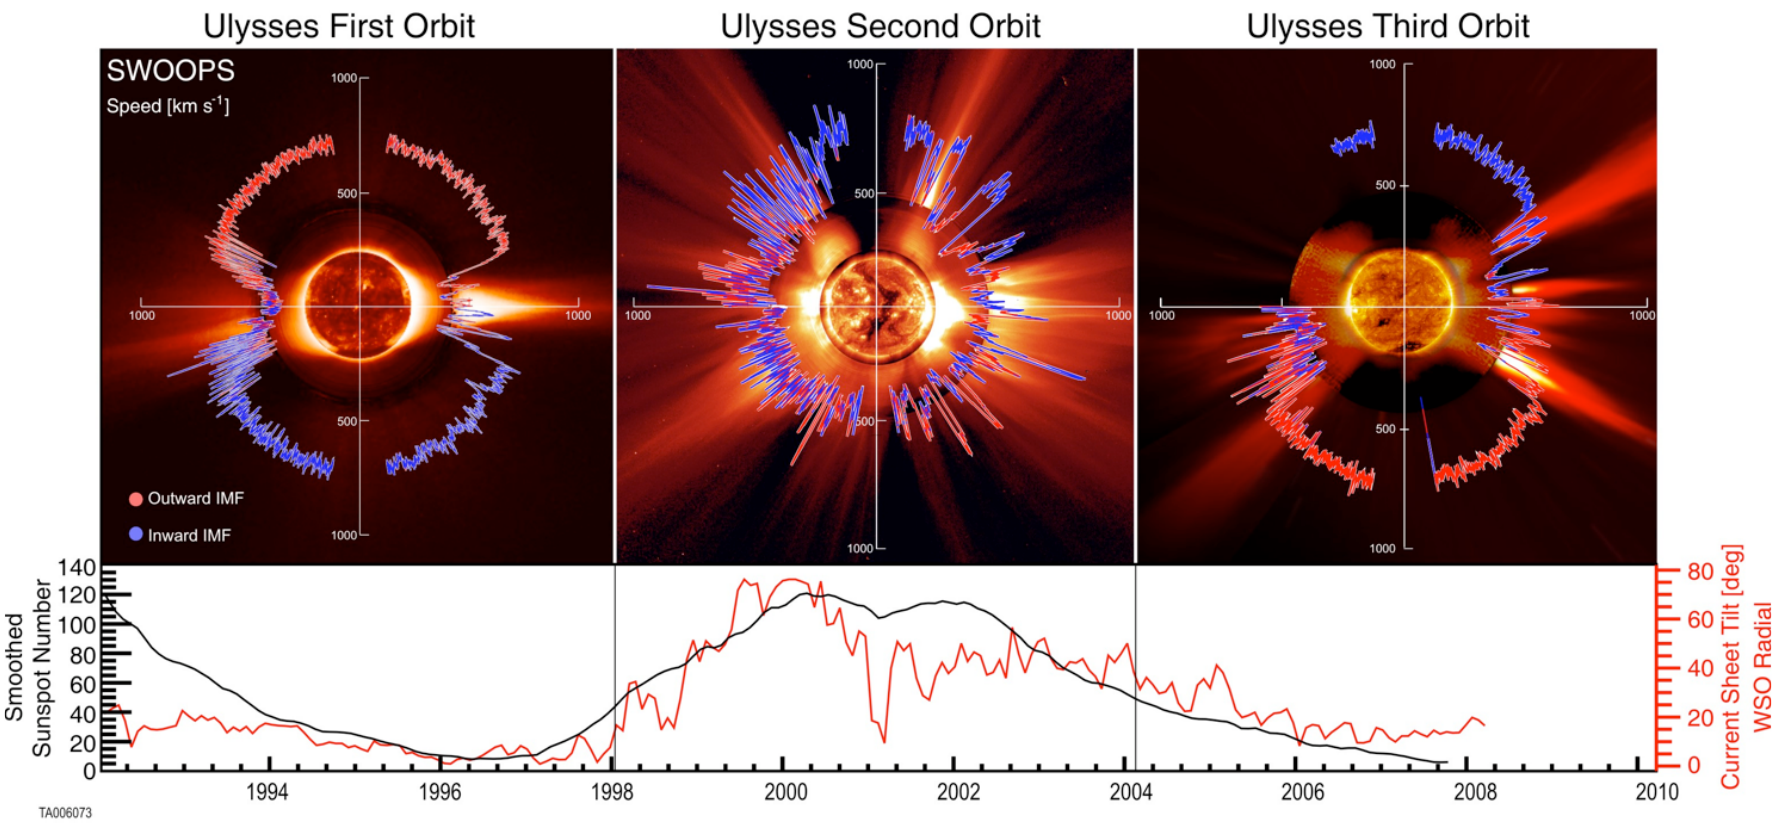
\includegraphics[width=0.9\textwidth]{../figures_of_others/images/McComas2008_Ulysses_orbit_.png}
	\captionoftiny{figure}{\centering Credit: {\citet[Fig.~1]{McComas200809}}}
\end{frame}

\begin{frame}[plain,c]{Coronal mass ejections}{}
	\begin{columns}[c]
	\column{0.5\textwidth}
	
		\onslide*<1-2>{
		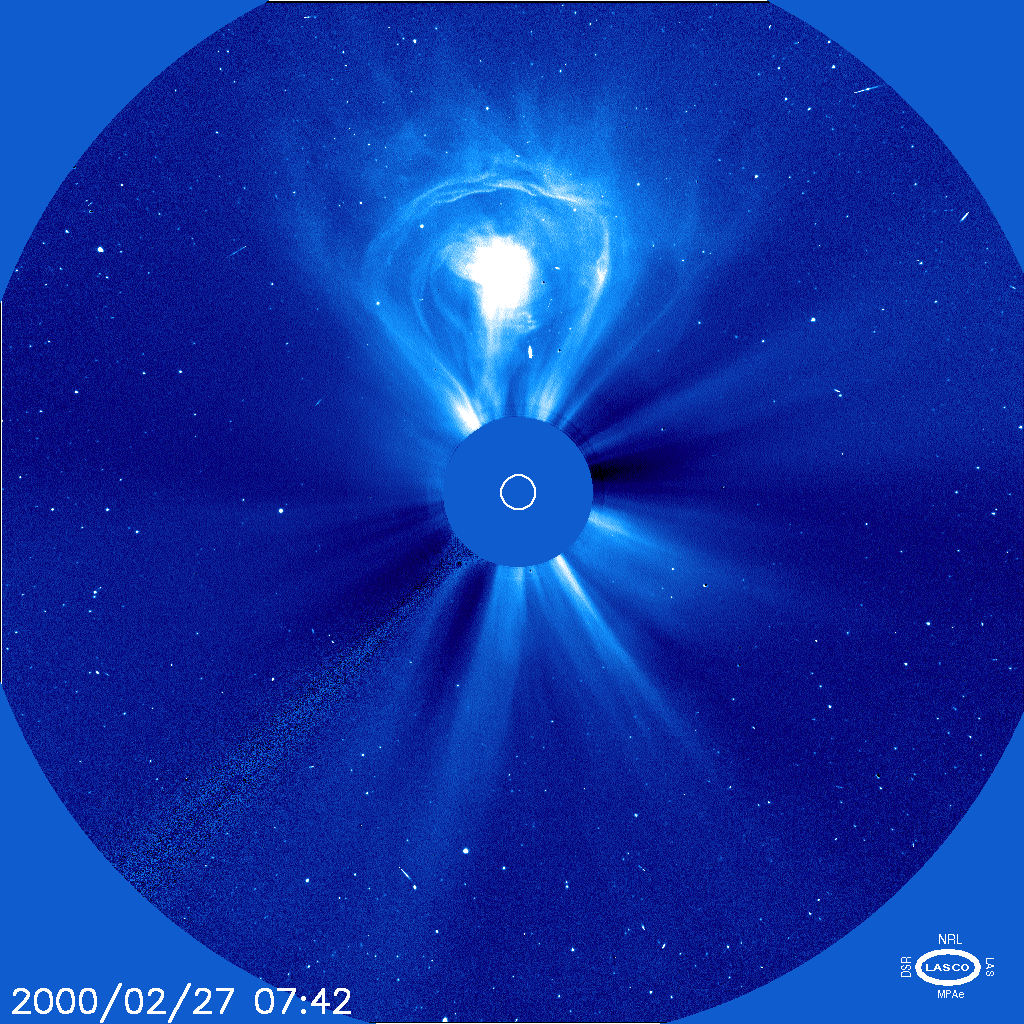
\includegraphics[height=\textwidth]{../figures_of_others/images/20000226_lightbulb_CME_c3full.png}
		\captionoftiny{figure}{Courtesy of SOHO/LASCO consortium. SOHO is a project of international cooperation between ESA and NASA}
		}
		\onslide*<3>{
		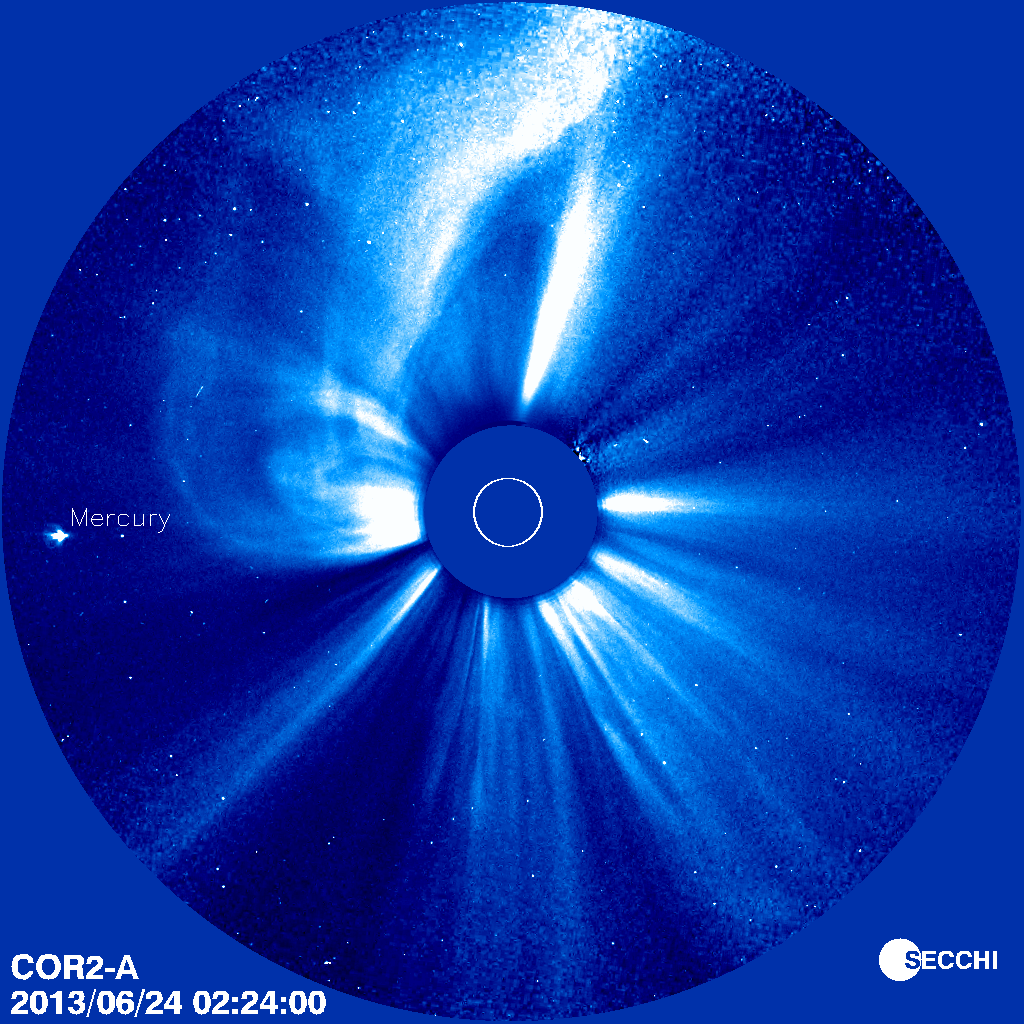
\includegraphics[height=\textwidth]{../figures_of_others/images/STEREO_A_COR2_20130624_022400_dbc2A.png}
		\captionoftiny{figure}{Courtesy of \href{https://stereo.gsfc.nasa.gov/gallery/copyright.shtml}{STEREO/COR2 consortium (NASA)}\\\ }
		}
		
		\onslide*<4>{
		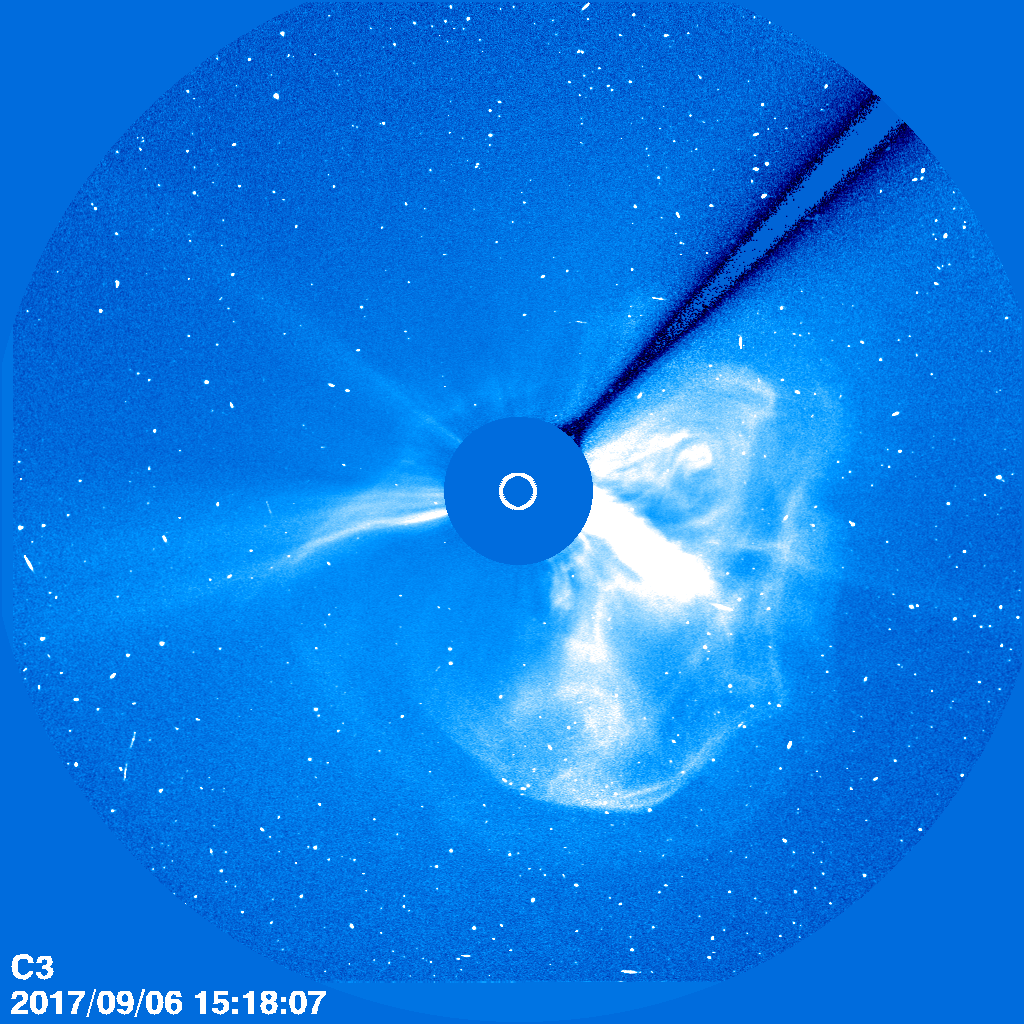
\includegraphics[height=\textwidth]{../figures_of_others/images/SOHO_LASCO_C3_20170906_151807.png}
		\captionoftiny{figure}{Courtesy of SOHO/LASCO consortium; SOHO is a project of international cooperation between ESA and NASA}
		}
	
	\column{0.05\textwidth}
	
	\column<2->{0.45\textwidth}

		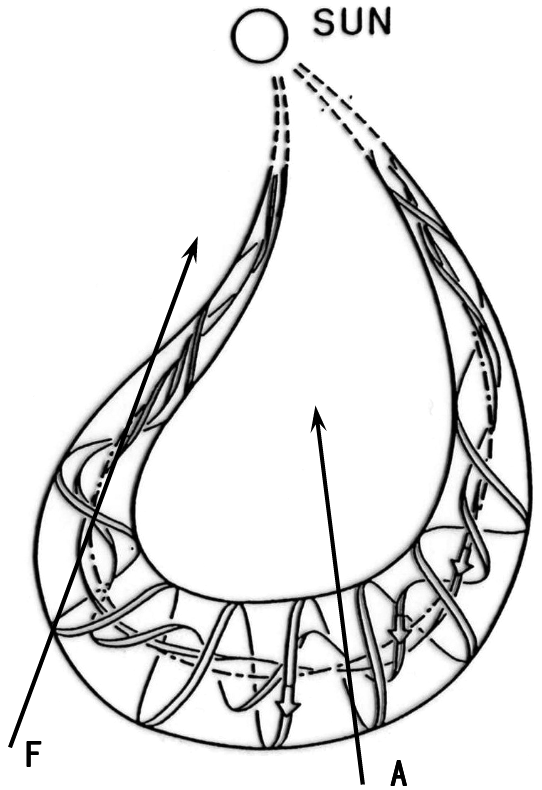
\includegraphics[height=0.9\textwidth]{../figures_of_others/images/Marubashi2007_fig1.png}
		\captionoftiny{figure}{\centering Credit: {\citet[Fig.~1, panel (a)]{Marubashi2007}}\\\ }
		
	\end{columns}
\end{frame}
\begin{frame}[plain,c]{CME orientation}{}
	\centering
	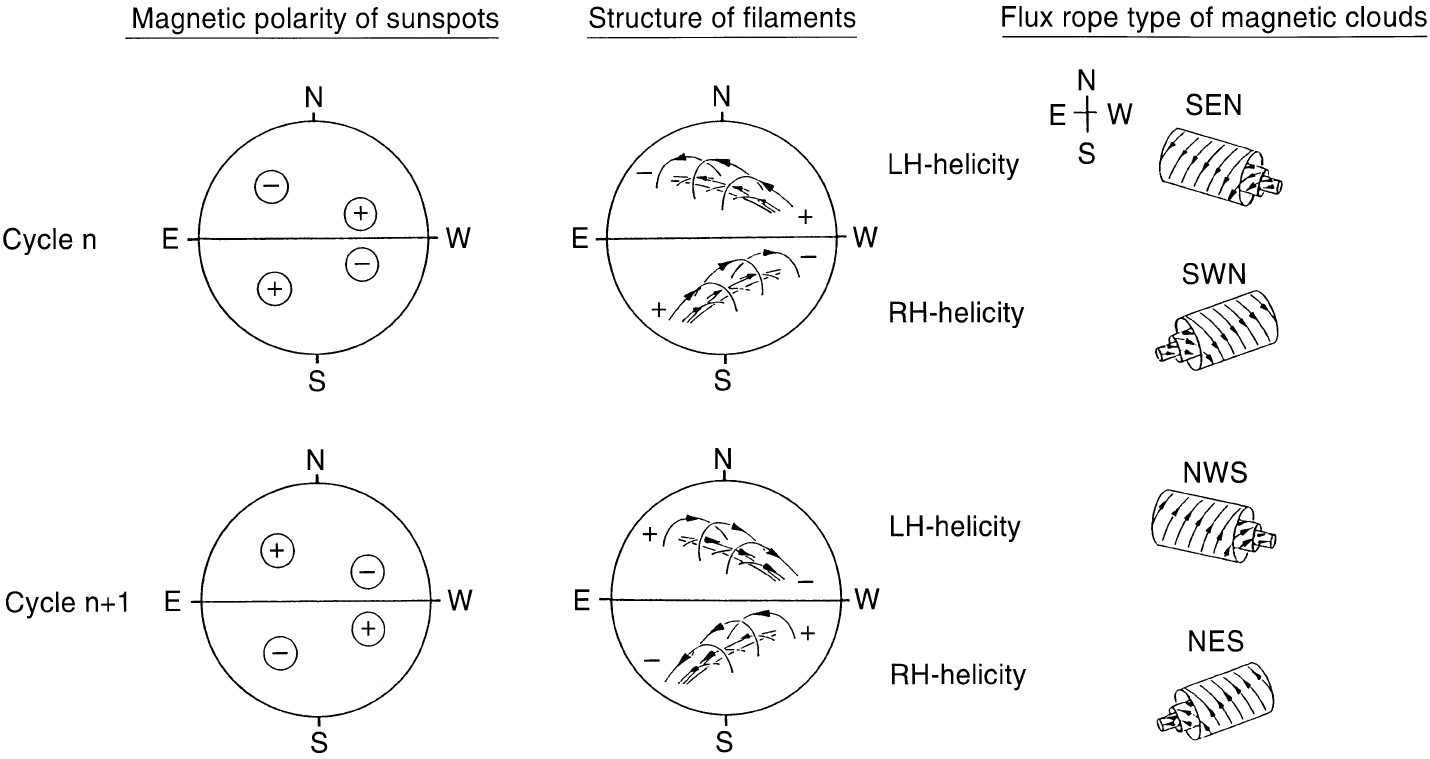
\includegraphics[width=0.9\textwidth]{../figures_of_others/images/Bothmer1998_fig18.png}
	\captionoftiny{figure}{\centering Credit: {\citet[Fig.~18]{Bothmer1998}}}
\end{frame}
\begin{frame}[plain,c]{In-situ CMEs}{}
	\centering
	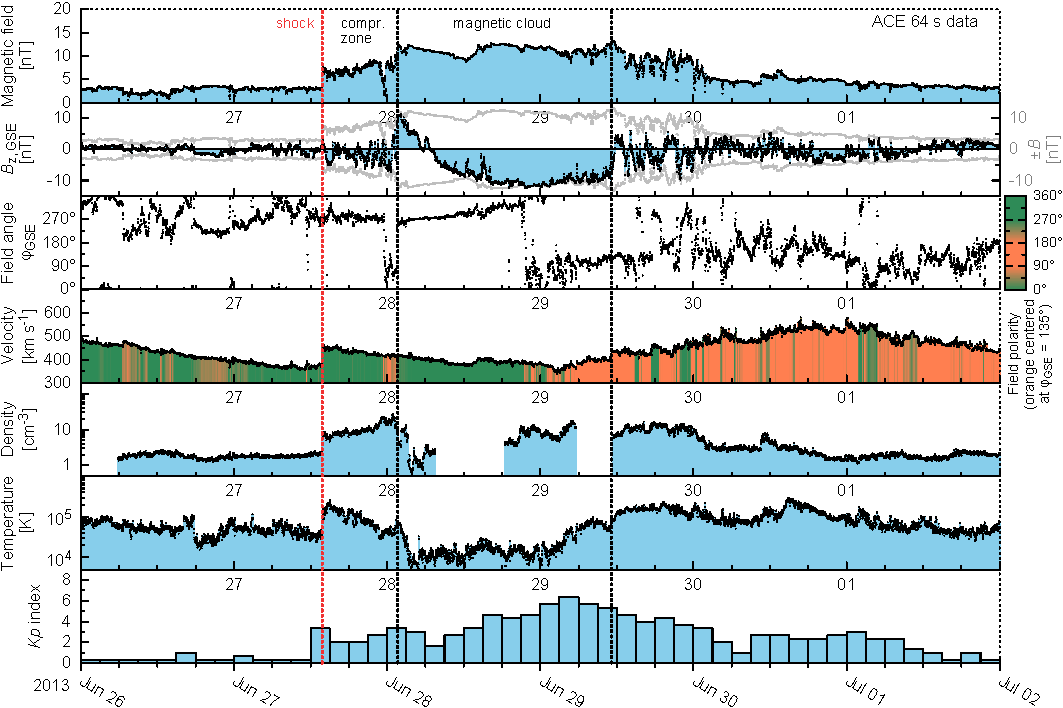
\includegraphics[width=0.8\textwidth]{../figures_of_mine/gnuplots/ACE_64s_v7_thesis_CME_2013-6-26_6.pdf}
\end{frame}
\begin{frame}[plain,c]{Solar wind and CME forecast}{}
	\centering
	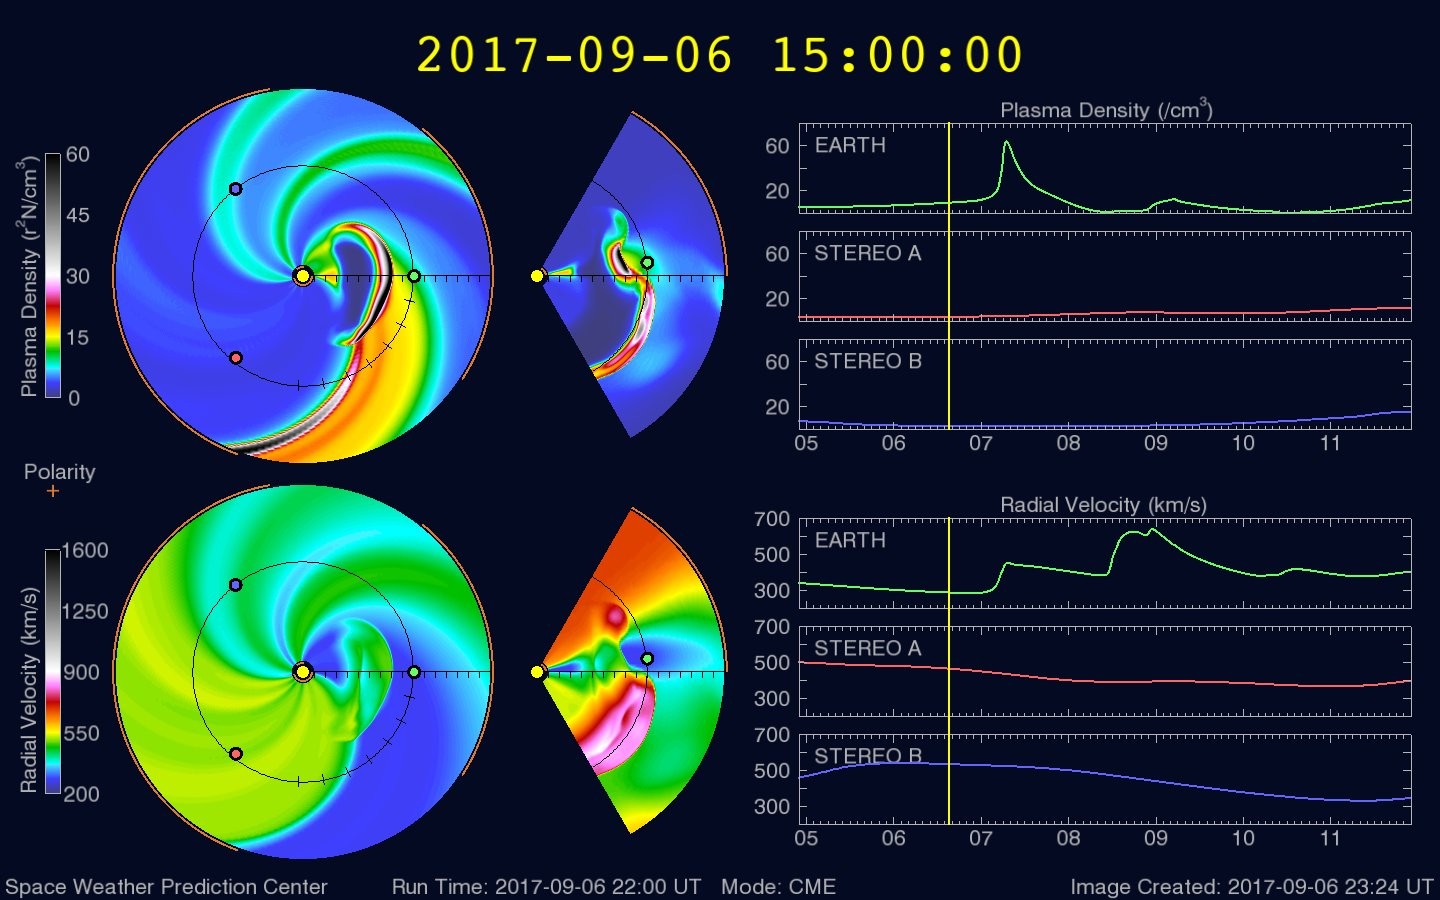
\includegraphics[width=0.8\textwidth]{../figures_of_others/images/enlil_com1_20170906T150000.jpg}
	\captionoftiny{figure}{\centering Credit: \href{http://dx.doi.org/10.7289/V5445JGH}{SWPC: WSA-Enlil Solar Wind Prediction. NOAA National Centers for Environmental Information}}
\end{frame}


\subsection{Chapter2}

\begin{frame}[plain,c]{\Kp{} long-term variations}{}
	\begin{columns}[c]
	\column{0.5\textwidth}
		
		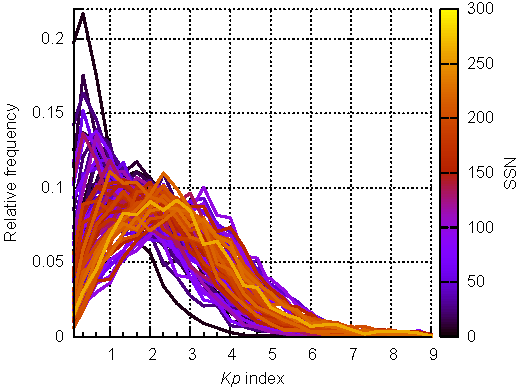
\includegraphics[width=\textwidth]{../figures_of_mine/chapter2/Kp_histogram_yearlySSN_b.pdf}
% 		\captionoftiny{figure}{}
		
	\column{0.5\textwidth}
		
		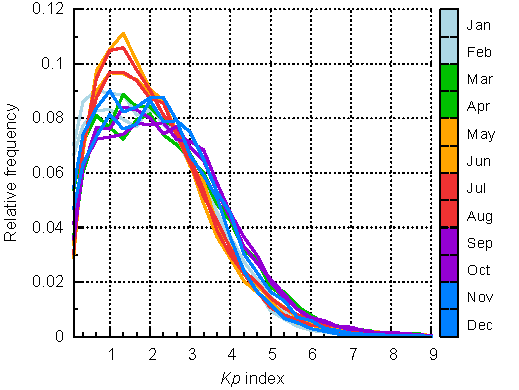
\includegraphics[width=\textwidth]{../figures_of_mine/chapter2/Kp_histogram_monthly.pdf}
% 		\captionoftiny{figure}{}
	\end{columns}
\end{frame}

\begin{frame}[c,label=prediction_performance]{Prediction performance}{}
	\begin{columns}[c]
	\column{0.5\textwidth}
		
		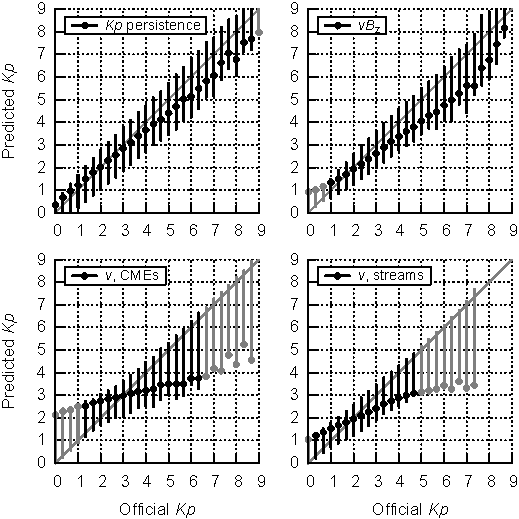
\includegraphics[width=\textwidth]{../figures_of_mine/chapter2/model_performance_d.pdf}
	
	\column{0.5\textwidth}

		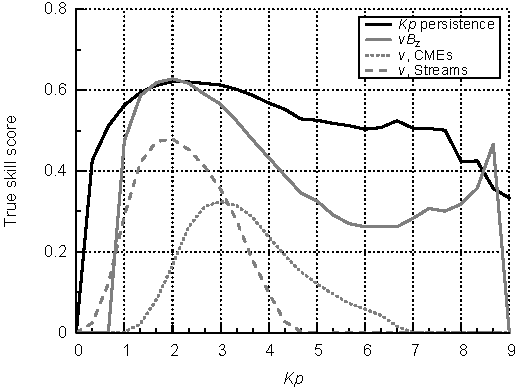
\includegraphics[width=\textwidth]{../figures_of_mine/chapter2/true_skill_score.pdf}
		
	\end{columns}
\end{frame}

\section{Geomagnetic impact of the solar wind}

\begin{frame}[plain,c]{Magnetosphere}{}
	\begin{columns}[c]
	\column{0.5\textwidth}
		
		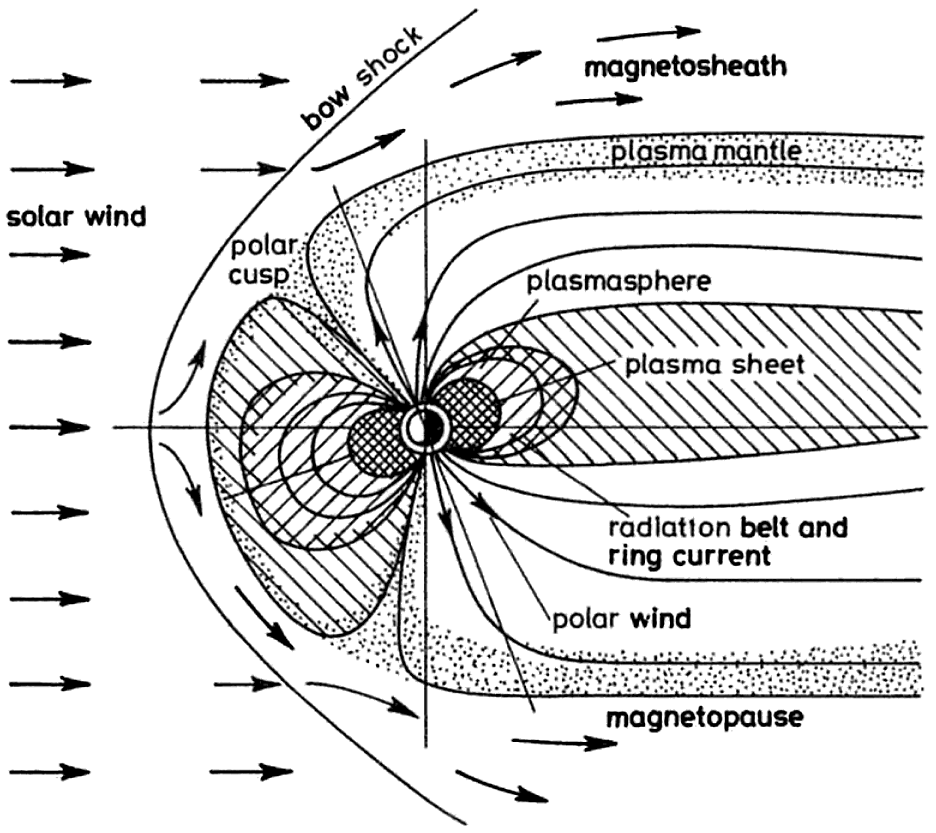
\includegraphics[width=\textwidth]{../figures_of_others/images/Davies1990_magnetosphere_sharpened.png}
		\captionoftiny{figure}{\centering Credit: {\citet[Fig.~2.12]{Davies1990}}}

	\column{0.5\textwidth}
		
		Interaction mechanisms between solar wind and magnetosphere:
		\begin{itemize}
			\item Reconnection
			\item Turbulence
			\item Compression
			\item Induction
		\end{itemize}

	\end{columns}
\end{frame}
\begin{frame}[plain,c]{Magnetosphere}{}
	\begin{columns}[c]
	\column{0.5\textwidth}
		
		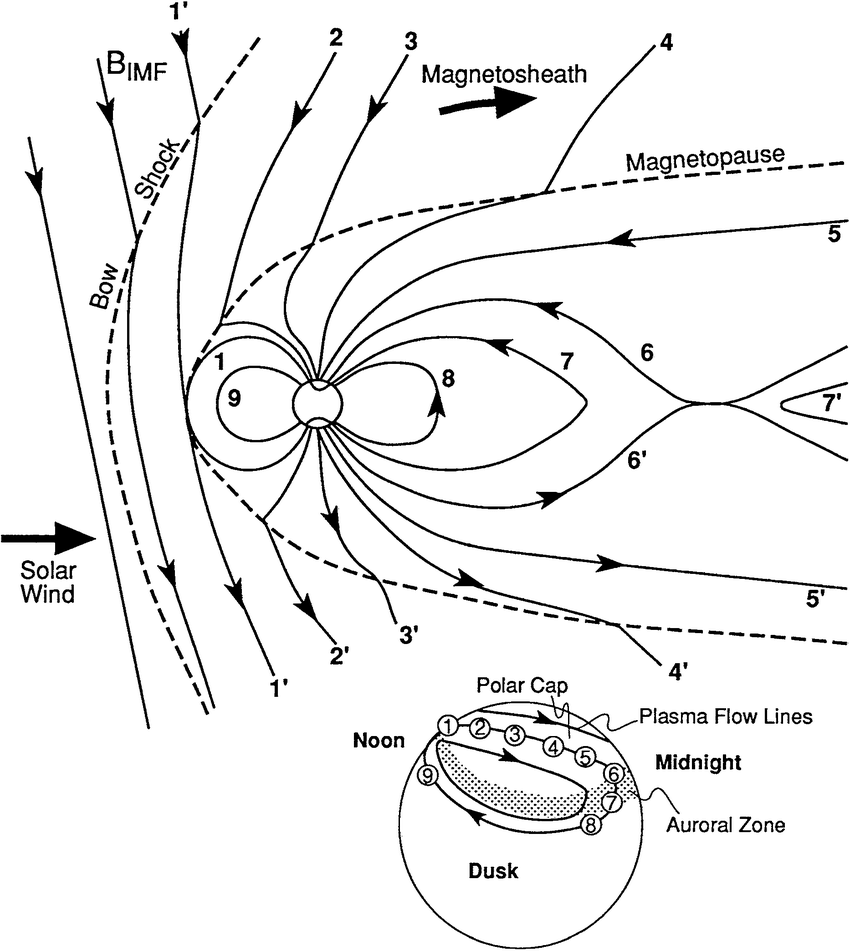
\includegraphics[width=\textwidth]{../figures_of_others/images/Kivelson1995_fig9_11_dungey_cycle.png}
		\captionoftiny{figure}{\centering Credit: {\citet[Fig.~9.11]{Hughes1995}}}
		
	\column{0.5\textwidth}
		
		Factors that influence the reconnection flux rate:
		\begin{itemize}
			\item Velocity
			\item Magnetic field strength
			\item Magnetic field angle
			\item Size of reconnection region
		\end{itemize}
		
	\end{columns}
\end{frame}
\begin{frame}[plain,c]{\Kp~index}{}
	\begin{columns}[c]
	\column{0.5\textwidth}
		
		- Planetary geomagnetic disturbance indicator\\
		- 3-hourly variation maxima\\
		- 13 observatories at \SI{50}{\degree} geomagnetic latitudes\\
		- Scale from 0 to 9
		
	\column{0.5\textwidth}
		
		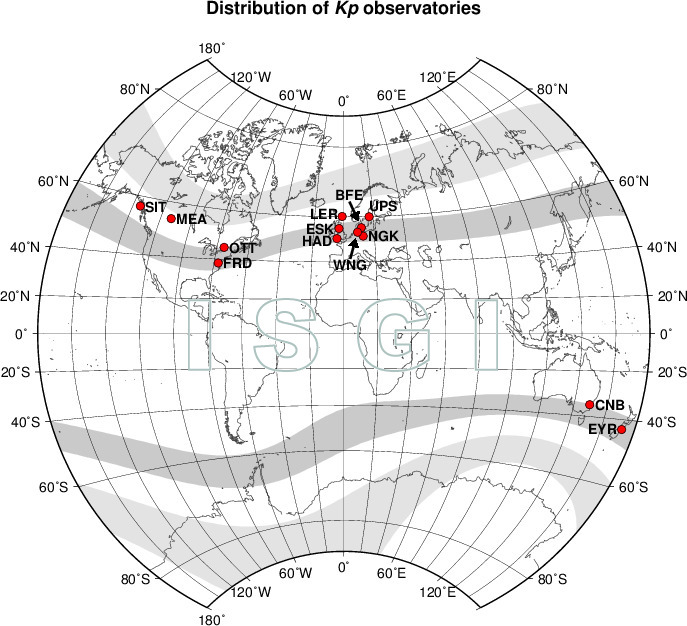
\includegraphics[width=\textwidth]{../figures_of_others/images/Kp_map.jpg}
		\captionoftiny{figure}{Courtesy of \href{http://isgi.unistra.fr/indices_kp.php}{International Service of Geomagnetic Indices (ISGI)}, 2013}
	\end{columns}
\end{frame}
\begin{frame}[plain,c]{\Kp~index}{Quicklook \Kp{}}
	\begin{columns}[c]
	\column{0.5\textwidth}
		
		\includegraphics[width=\textwidth]{../talk_figures/ql_bar.png}
		\captionoftiny{figure}{\centering Credit: \href{http://www.gfz-potsdam.de/en/kp-index/}{GFZ~Potsdam}, 2018}
	\end{columns}
\end{frame}

\begin{frame}[plain,c]{Solar wind electric field}{}
	\begin{columns}[c]
	\column{0.5\textwidth}
		
% 		\includegraphics[width=\textwidth]{../figures_of_mine/chapter2/histogram_VBzgsm.pdf}
	
	\column{0.5\textwidth}

		\includegraphics[width=\textwidth]{../figures_of_mine/chapter2/cc_lag_data_d_KpvsVBzgsm.pdf}
		
	\end{columns}
\end{frame}
\begin{frame}[plain,c]{Solar wind electric field}{}
	\begin{columns}[c]
	\column{0.5\textwidth}
		
		\includegraphics[width=\textwidth]{../figures_of_mine/chapter2/Kp_2dhistogram_VBzgsm_sws_e.pdf}
	
	\column{0.5\textwidth}

		\includegraphics[width=\textwidth]{../figures_of_mine/chapter2/Kp_2dhistogram_VBzgsm_sws_fit_e.pdf}
		
	\end{columns}
\end{frame}
\begin{frame}[plain,c]{Solar wind velocity}{}
	\begin{columns}[c]
	\column{0.5\textwidth}
		
% 		\includegraphics[width=\textwidth]{../figures_of_mine/chapter2/histogram_V_d.pdf}
	
	\column{0.5\textwidth}

		\includegraphics[width=\textwidth]{../figures_of_mine/chapter2/cc_lag_sws_f.pdf}
		
	\end{columns}
\end{frame}

\begin{frame}[plain,c]{Solar wind velocity}{}
	\begin{columns}[c]
	\column{\textwidth}
		
		\centering
		\includegraphics[width=0.9\textwidth]{../figures_of_mine/chapter2/Kp_2dhistogram_V_sws_e.pdf}

	\end{columns}
\end{frame}
\begin{frame}[plain,c]{}{}
	\begin{columns}[c]
	\column{0.5\textwidth}
		
% 		\includegraphics[width=\textwidth]{../figures_of_mine/chapter2/histogram_V_d.pdf}
	
	\column{0.5\textwidth}

		\includegraphics[width=\textwidth]{../figures_of_mine/chapter2/cc_lag_sws_f.pdf}
		
	\end{columns}
\end{frame}

\begin{frame}[plain,c]{CME velocity}{}
	\begin{columns}[c]
	\column{0.5\textwidth}
		
		\includegraphics[width=\textwidth]{../figures_of_mine/chapter2/Kp_2dhistogram_V_sws1_d.pdf}
	
	\column{0.5\textwidth}

		\includegraphics[width=\textwidth]{../figures_of_mine/chapter2/Kp_2dhistogram_V_sws1_fit_e.pdf}
		
	\end{columns}
\end{frame}
\begin{frame}[plain,c]{Stream velocity}{}
	\begin{columns}[c]
	\column{0.5\textwidth}
		
		\includegraphics[width=\textwidth]{../figures_of_mine/chapter2/Kp_2dhistogram_V_sws23_e.pdf}
	
	\column{0.5\textwidth}

		\includegraphics[width=\textwidth]{../figures_of_mine/chapter2/Kp_2dhistogram_V_sws23_fit_e.pdf}
		
	\end{columns}
\end{frame}
\begin{frame}[plain,c]{}{}
	\begin{columns}[c]
	\column{\textwidth}
		
		\centering
		\includegraphics[width=0.8\textwidth]{../figures_of_mine/chapter2/example_sw_plot_1month_b_9hshift_2013-5-1_65.pdf}
	
	\end{columns}
\end{frame}
\begin{frame}[plain,c]{}{}
	\begin{columns}[c]
	\column{\textwidth}
		\centering
		\includegraphics[width=0.8\textwidth]{../figures_of_mine/chapter2/example_sw_plot_CME_b_9hshift_2013-6-26_6.pdf}
	
	\end{columns}
\end{frame}

\begin{frame}[plain,c]{Results}{}
	\begin{columns}[c]
	\column{\textwidth}
		
		Predictive \Kp{} models based on relations with
		\begin{itemize}%[<+->]
			\item Solar wind electric field proxy (\vBz{})
			\item Velocity of CME-associated flows ($v_\text{CME}$)
			\item Velocity of solar wind streams ($v_\text{stream}$)
		\end{itemize}
		
	\end{columns}
\end{frame}
\begin{frame}[plain,c]{Conclusions}{}
% 	\begin{columns}[c]
% 	\column{\textwidth}
		
		\begin{itemize}%[<+->]
			\item The processing of 3-hour extrema of high time resolution data captures short-term geoeffective magnetic features that are neglected when averaging over 3-hour intervals
			\item The isolated treatment of CMEs and streams is beneficial to the prediction accuracy of \Kp{}
			\item The prediction models perform well for their limited input information
		\end{itemize}
		
% 	\end{columns}
	
	\vspace*{\fill} \hfill \hyperlink{prediction_performance}{\beamerskipbutton{Prediction performance}}
\end{frame}


\section{Solar wind model for the inner heliosphere}

\begin{frame}[c,label=lognormal_distribution]{Lognormal distribution}{}
	\begin{columns}[c]
	\column{0.5\textwidth}
		
		\includegraphics[width=\textwidth]{../figures_of_mine/gnuplots/lognormal_semi_log.pdf}

	\column{0.5\textwidth}
	
		\small Probability density function:
		\begin{align}
			f(x) &= \frac{1}{\sigma \sqrt{2 \pi} x} \, \text{e}^{- \frac{(\ln x - \mu)^2}{2 \sigma^2}}	\nonumber
		\end{align}
		Location ($\mu$) and shape parameter ($\sigma$).\\\ \\
		Median and average:
		\begin{align}
			x_\text{med} = \exp\left(\mu\right)\,,	&	&	x_\text{avg} = \exp\left(\mu + \frac{\sigma^2}{2}\right)	\nonumber
		\end{align}
		\begin{align}
			f(x) = \frac{1}{2 \sqrt{\pi \ln\left(\frac{x_\text{avg}}{x_\text{med}}\right)} \, x} \, \exp\left(- \frac{\ln^2\left(\frac{x}{x_\text{med}}\right)}{4 \ln\left(\frac{x_\text{avg}}{x_\text{med}}\right)}\right)	\nonumber
		\end{align}

	\end{columns}
\end{frame}
\begin{frame}[plain,c]{Near-Sun region}{}
	Unsolved problems:	
	- Coronal heating mechanisms\\
	- Solar wind acceleration processes\\
	- Solar energetic particle sources
\end{frame}
\begin{frame}[plain,c]{Solar activity}{}
	\begin{columns}[c]
	\column{0.5\textwidth}
		
		\includegraphics[width=\textwidth]{../figures_paper/OMNI_yearly_BVNTvsSSN_a.pdf}

	\column{0.5\textwidth}

		\includegraphics[width=\textwidth]{../figures_paper/Vdbl_SSN_ratio_f_plot.pdf}

	\end{columns}
\end{frame}
\begin{frame}[plain,c]{PSP perihelia prediction}{}
	\centering
	\includegraphics[width=0.8\textwidth]{../figures_paper/SPP_sw_distributions_b.pdf}
\end{frame}



% 
\section{Test slides}

\begin{frame}[c]{first slide}{A bit more information about this}
	This is a text in first frame. \pause This is a text in first frame. This is a text in first frame.
	\begin{definition}
		A definition
	\end{definition}
	\url{https://www.sharelatex.com/learn/latex/Beamer}
\end{frame}

\begin{frame}[<+->]{Ein Demotitel}{}
	\begin{itemize}
		\item<1-> dasgfs
		\item<2> asgag
		\item<3-> asgag
		\item asgag
	\end{itemize}
\end{frame}

\begin{frame}[<+->]{Ein Demotitel}{}
	\begin{itemize}
		\item dasgfs
		\item asgag
		\item asgag
		\item<.-> asgag
	\end{itemize}
\end{frame}

\begin{frame}{Ein Demotitel}{}
	\begin{itemize}
		\item<+-> dasgfs
		\item<+-> asgag
		\item<+-> asgag
		\item<+-> asgag
	\end{itemize}
\end{frame}
\begin{frame}{Ein Demotitel}{}
	\begin{itemize}[<+->]
		\item dasgfs
		\item asgag
		\item asgag
		\item asgag
	\end{itemize}
\end{frame}

\section{part two}

\begin{frame}[t]{Sample frame title}{}
	
	In this slide, some important text will be
	\alert<2->{highlighted} beause it's important.
	Please, don't abuse it.
	
	\onslide<2>{	%\uncover{}
	\begin{block}{Remark}
	Sample text
	\end{block}
	}
	
	\onslide*<1>{	%\only{}
	\begin{examples}
	Sample text in green box. "Examples" is fixed as block title.
	\end{examples}
	}
	
	\onslide+<2>{	%\visible{}
	\begin{alertblock}{Important theorem}
	Sample text in red box
	\end{alertblock}
	}
	
\end{frame}

\begin{frame}[plain]{Sample frame title}{}
	
	In this slide, some important text will be
	\alert{highlighted} beause it's important.
	Please, don't abuse it.
	
	\begin{block}{Remark}
	Sample text
	\end{block}
	
	\begin{alertblock}{Important theorem}
	Sample text in red box
	\end{alertblock}
	
	\begin{examples}
	Sample text in green box. "Examples" is fixed as block title.
	\end{examples}
\end{frame}

\section{part 3}

\begin{frame}{Two-column slide}{}
	\begin{columns}[t]
		\column{0.5\textwidth}
		This is a text in first column.
		$$E=mc^2$$
		\begin{itemize}
		\item First item
		\item Second item
		\end{itemize}
		
		\column{0.5\textwidth}
		This text will be in the second column
		and on a second tought this is a nice looking
		layout in some cases \citep{Venzmer2018}.
	\end{columns}
\end{frame}

\begin{frame}[t]{Sample}{}
	
	In this slide, some important text will be
	\alert<2->{highlighted} beause it's important.
	Please, don't abuse it.
	
	\begin{block}<1->{Remark}
	Sample text
	\end{block}
	
	\begin{examples}<2>
	Sample text in green box. "Examples" is fixed as block title.
	\end{examples}
	
	\begin{alertblock}<3>{Important theorem}
	Sample text in red box
	\end{alertblock}
	
\end{frame}

\section{Backup slides 2}

\begin{frame}{backup slide}{}
	gj
	
	\hyperlink{butterfly}{\beamerbutton{Magnetic butterfly diagram}}
	
	\hyperlink{butterfly}{\beamergotobutton{Go to my frame}}
	
	\hyperlink{butterfly}{\beamerreturnbutton{Back}}
	
	\hyperlink{butterfly}{\beamerskipbutton{butterfly page}}
\end{frame}

% \begin{frame}[]{title}{subtitle}
%
% \end{frame}
 



\end{document}


